\documentclass{beamer}

\usepackage{graphicx}
\graphicspath{{figuras/}}
\usetheme{Madrid}
\setbeamertemplate{navigation symbols}{}
\setbeamertemplate{caption}[numbered]
\usepackage{verbatim}
\usepackage{caption}   %para subfiguras
\usepackage{subcaption}%para subfiguras
%%%%%%%%%%%%%%%%%%%%%%%%%%%%%%%%%%%%%%%%%%%%%%%%%%%%%%
\usepackage[utf8]{inputenc}    %esses tres sao
\usepackage[T1]{fontenc}       %necessarios
\usepackage[portuguese]{babel} %para usar palavras com acento
%%%%%%%%%%%%%%%%%%%%%%%%%%%%%%%%%%%%%%%%%%%%%%%%%%%%%%
\usepackage[]{mathtools}
\usepackage{siunitx}

% \usepackage[linesnumbered, ruled, figure, portuguese]{algorithm2e}
% \SetKwBlock{Inicio}{Início}{Fim}
% \SetKwFor{ParaCada}{para cada}{faça}{fim para}
% \usepackage{listings}

% \lstset{
%   language=Python,
%   showstringspaces=false,
%   formfeed=newpage,
%   tabsize=4,
%   basicstyle=\footnotesize
% }

%\usefonttheme{serif}
%\renewcommand\rmdefault{phv}
%\usepackage{arev}
%\usepackage[sfmath]{kpfonts}

\usepackage[authoryear]{natbib}
\bibliographystyle{apalike}

%*****************************************************
\makeatletter
\setbeamertemplate{footline}
{
  \leavevmode%
  \hbox{%
  \begin{beamercolorbox}[wd=.333333\paperwidth,ht=2.25ex,dp=1ex,center]{title in head/foot}%
    \usebeamerfont{author in head/foot}Gabriel Lauffer Ramos%~~\beamer@ifempty{\insertshortinstitute}{}{(\insertshortinstitute)}
  \end{beamercolorbox}%
  \begin{beamercolorbox}[wd=.333333\paperwidth,ht=2.25ex,dp=1ex,center]{title in head/foot}%
    \usebeamerfont{title in head/foot}TCC II
  \end{beamercolorbox}%
  \begin{beamercolorbox}[wd=.333333\paperwidth,ht=2.25ex,dp=1ex,right]{title in head/foot}%
    \usebeamerfont{date in head/foot}\texttt{24 de junho de 2016}\hspace*{2em}
    \insertframenumber{} / \inserttotalframenumber\hspace*{2ex}
  \end{beamercolorbox}}%
  \vskip0pt%
}
\makeatother
%************************************************************
\institute{Universidade Federal do Rio Grande - FURG\\
Instituto de Matemática, Estatística e Física - IMEF \\
Grupo de Astrofísica Teórica e Computacional - GATC}

\title{Determinação de Pulsação Estelar Através da Entropia de Shannon Condicional.}
%\subtitle{Trabalho de Conclusão de Curso}

\author{Gabriel Lauffer Ramos \\
Orientador: Fabricio Ferrari}

\date{Trabalho de Conclusão de Curso}
% - Either use conference name or its abbreviation.
% - Not really informative to the audience, more for people (including
%   yourself) who are reading the slides online

%\subject{Theoretical Computer Science}
% This is only inserted into the PDF information catalog. Can be left
% out.

% If you have a file called "university-logo-filename.xxx", where xxx
% is a graphic format that can be processed by latex or pdflatex,
% resp., then you can add a logo as follows:

% \pgfdeclareimage[height=0.5cm]{university-logo}{university-logo-filename}
% \logo{\pgfuseimage{university-logo}}

% Delete this, if you do not want the table of contents to pop up at
% the beginning of each subsection:
%\AtBeginSubsection[]
%{
 % \begin{frame}<beamer>{Outline}
  %  \tableofcontents[currentsection,currentsubsection]
  %\end{frame}
%}

% Let's get started

\begin{document}

%%%%%%%%%%%%%%%%%%%%%%%%%%%%%%%%%%%%%%%%%%%%%%%%%%%%%
\begin{frame}
  \titlepage
\end{frame}

%%%%%%%%%%%%%%%%%%%%%%%%%%%%%%%%%%%%%%%%%%%%%%%%%%%%%%
%\begin{frame}{Outline}
%  \tableofcontents
%  % You might wish to add the option [pausesections]
%\end{frame}

% Section and subsections will appear in the presentation overview
% and table of contents.
%%%%%%%%%%%%%%%%%%%%%%%%%%%%%%%%%%%%%%%%%%%%%%%%%%%%%%

%-----------------------------------------------------------------------
\section{Introdução}
%-----------------------------------------------------------------------

\begin{frame}[allowframebreaks]{Introdução}
  \begin{itemize}
    \item Estrelas variáveis são estrelas cuja a magnitude varia com o tempo.
    \item Determinar o período de variação da magnitude é fundamental para descrever a estrela.
    \begin{itemize}
%\item Luminosidade
%\item Massa
    \item Distância \citep{Leavitt1912}.
    \item Densidade média \citep{Payne1930}.
  \end{itemize}
  \item Porém, dependendo das condições climáticas e da disponibilidade do telescópio, nem sempre temos acesso a dados com uma variação temporal constante.
\end{itemize}

\framebreak


\begin{figure}
  \centering
  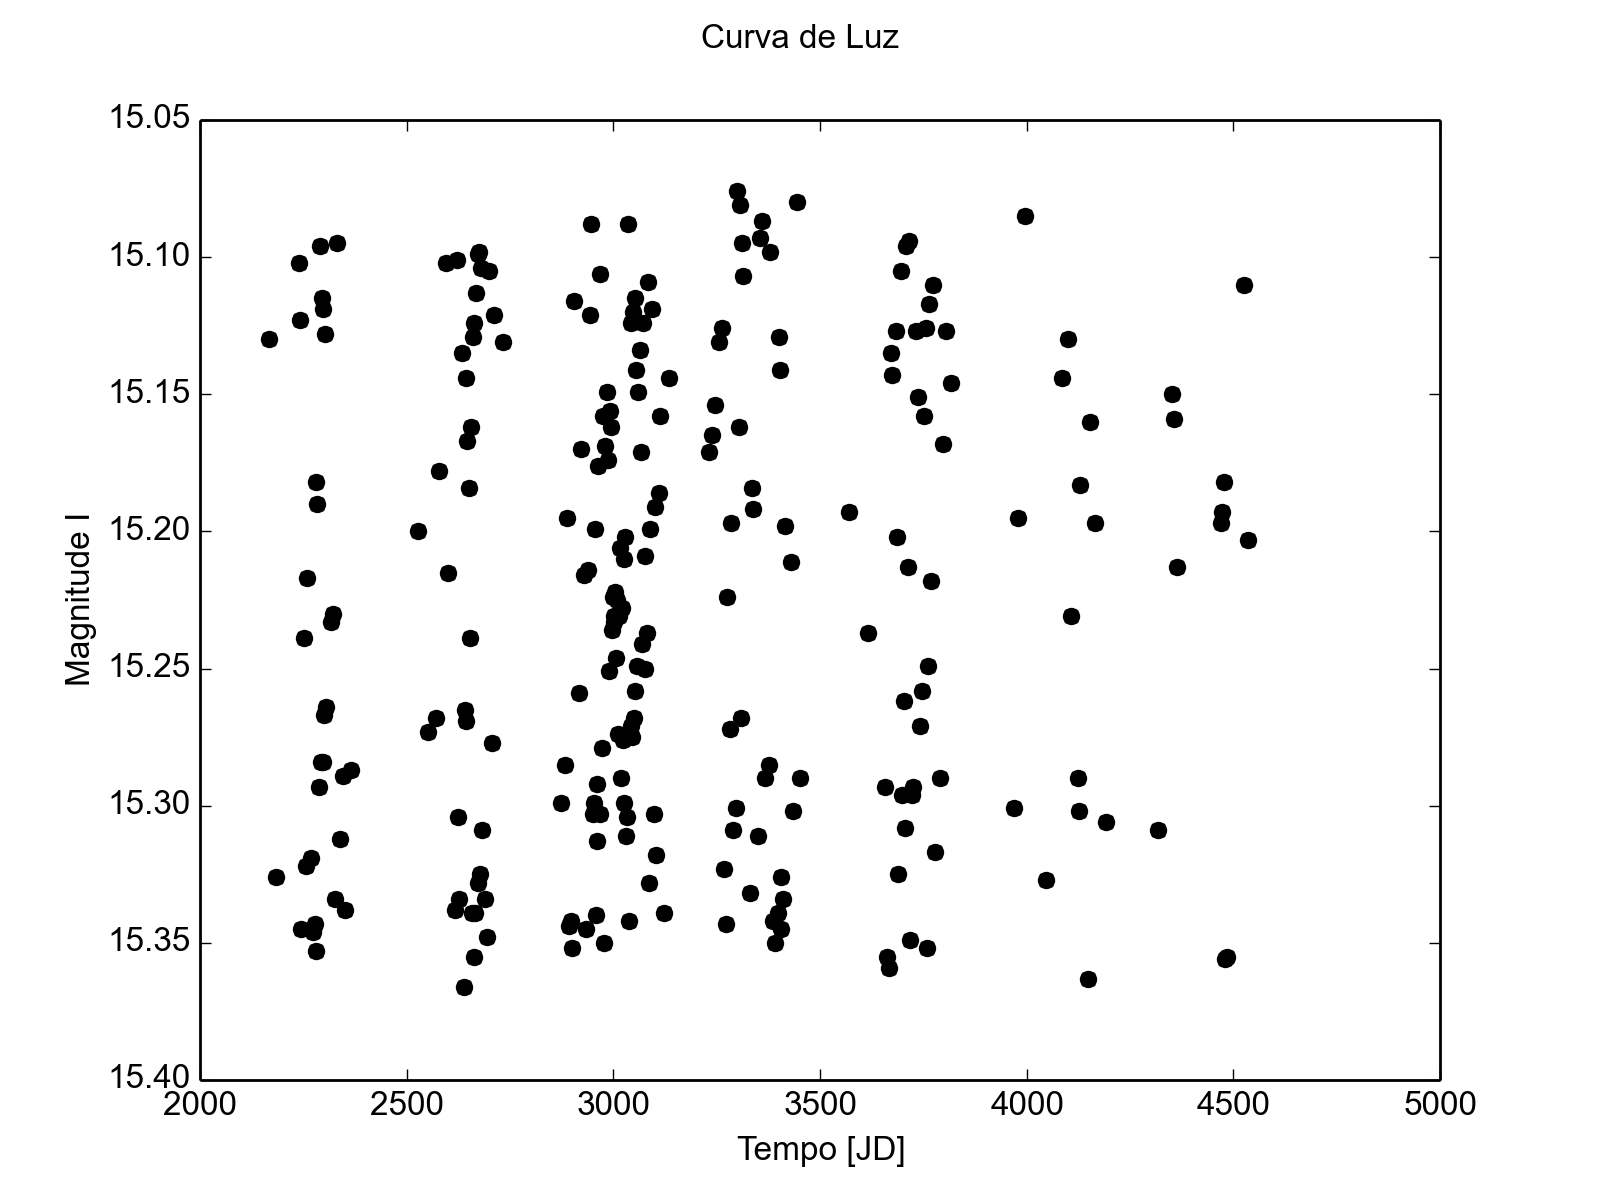
\includegraphics[scale=0.4]{0018_curva.png}
  \caption{Exemplo de dados obtidos do Catálogo OGLE-III para uma Cefeida Clássica.}
  \label{fig:ogle}
\end{figure}

\framebreak

\begin{itemize}
  \item Existem diversos métodos que lidam com dados igualmente espaçados.
    \begin{itemize}
    \item Análise de Fourier \citep{mello81,lomb}
  \end{itemize}
  \item Existem alguns métodos para lidar com dados que não possuam variação temporal constante.
  \begin{itemize}
    \item Análise do espaço de fase \citep{aov,entropy,Cincotta1999,ce}
  \end{itemize}
  \item Nenhum método se sobressai em relação aos outros \citep{comparison}.
%\item Objetivo: Testar um método que funcione tanto em dados com variação temporal constante e variável, baseado na entropia de Shannon condicional.
\end{itemize}

\end{frame}

%-----------------------------------------------------------------------
\section{Objetivo}
%-----------------------------------------------------------------------

\begin{frame}{Objetivo}
O objetivo deste trabalho é testar um algoritmo que seja confiável para trabalhar com séries temporais astronômicas e que não seja dependente do espaçamento
entre os dados observacionais.
  \begin{itemize}
    \item Este algoritmo trabalha com a entropia de Shannon condicional \citep{Cincotta1999,ce}, um método que utiliza a dispersão no espaço de fase para obter o período da série temporal através da minimização da entropia
  \end{itemize}
\end{frame}


%-----------------------------------------------------------------------
\section{Estrelas Variáveis}
%-----------------------------------------------------------------------

\begin{frame}{Estrelas Variáveis}
  \begin{itemize}
    \item Estrelas cuja magnitude varia com o tempo
    \item Classificadas em dois grandes grupos:
    \begin{itemize}
      \item \textit{\textbf{Variáveis Intrínsecas}}
      \item \textit{\textbf{Variáveis Extrínsecas}}
    \end{itemize}
  \end{itemize}

%   \begin{columns}
%     \begin{column}{0.45\textwidth}
%     \center{\textit{\textbf{Variáveis Intrínsecas}}} \\
%     \begin{itemize}
%       \item Processos internos
%       \begin{itemize}
%         \item Pulsantes
%         \item Eruptivas
%         \item Cataclísmicas
%       \end{itemize}
%     \end{itemize}
%   \end{column}

% \begin{column}{0.45\textwidth}
% \vspace{-0.55cm}
% \center{\textit{\textbf{Variáveis Extrínsecas}}}
% \begin{itemize}
% \item Processos externos
% \begin{itemize}
% \item Sistemas binários
% \item Rotação
% \end{itemize}
% \end{itemize}
% \end{column}

% \end{columns}
\end{frame}


\begin{frame}{Variáveis Extrínsecas}
\begin{itemize}
  \item Variação da luminosidade causada por algum processo externo.
  \begin{itemize}
    \item Variáveis eclipsantes
    \item Variáveis rotacionais
  \end{itemize}
\end{itemize}
\end{frame}

% \begin{frame}{Variáveis Extrínsecas - Eclipsantes}
% \begin{itemize}
%   \item Esta subclassificação incluí os sistemas binários de estrelas e variações na magnitude devido a asteroides ou exoplanetas.
% \end{itemize}

% \begin{figure}
% \centering
% \begin{subfigure}{.5\textwidth}
%   \centering
%   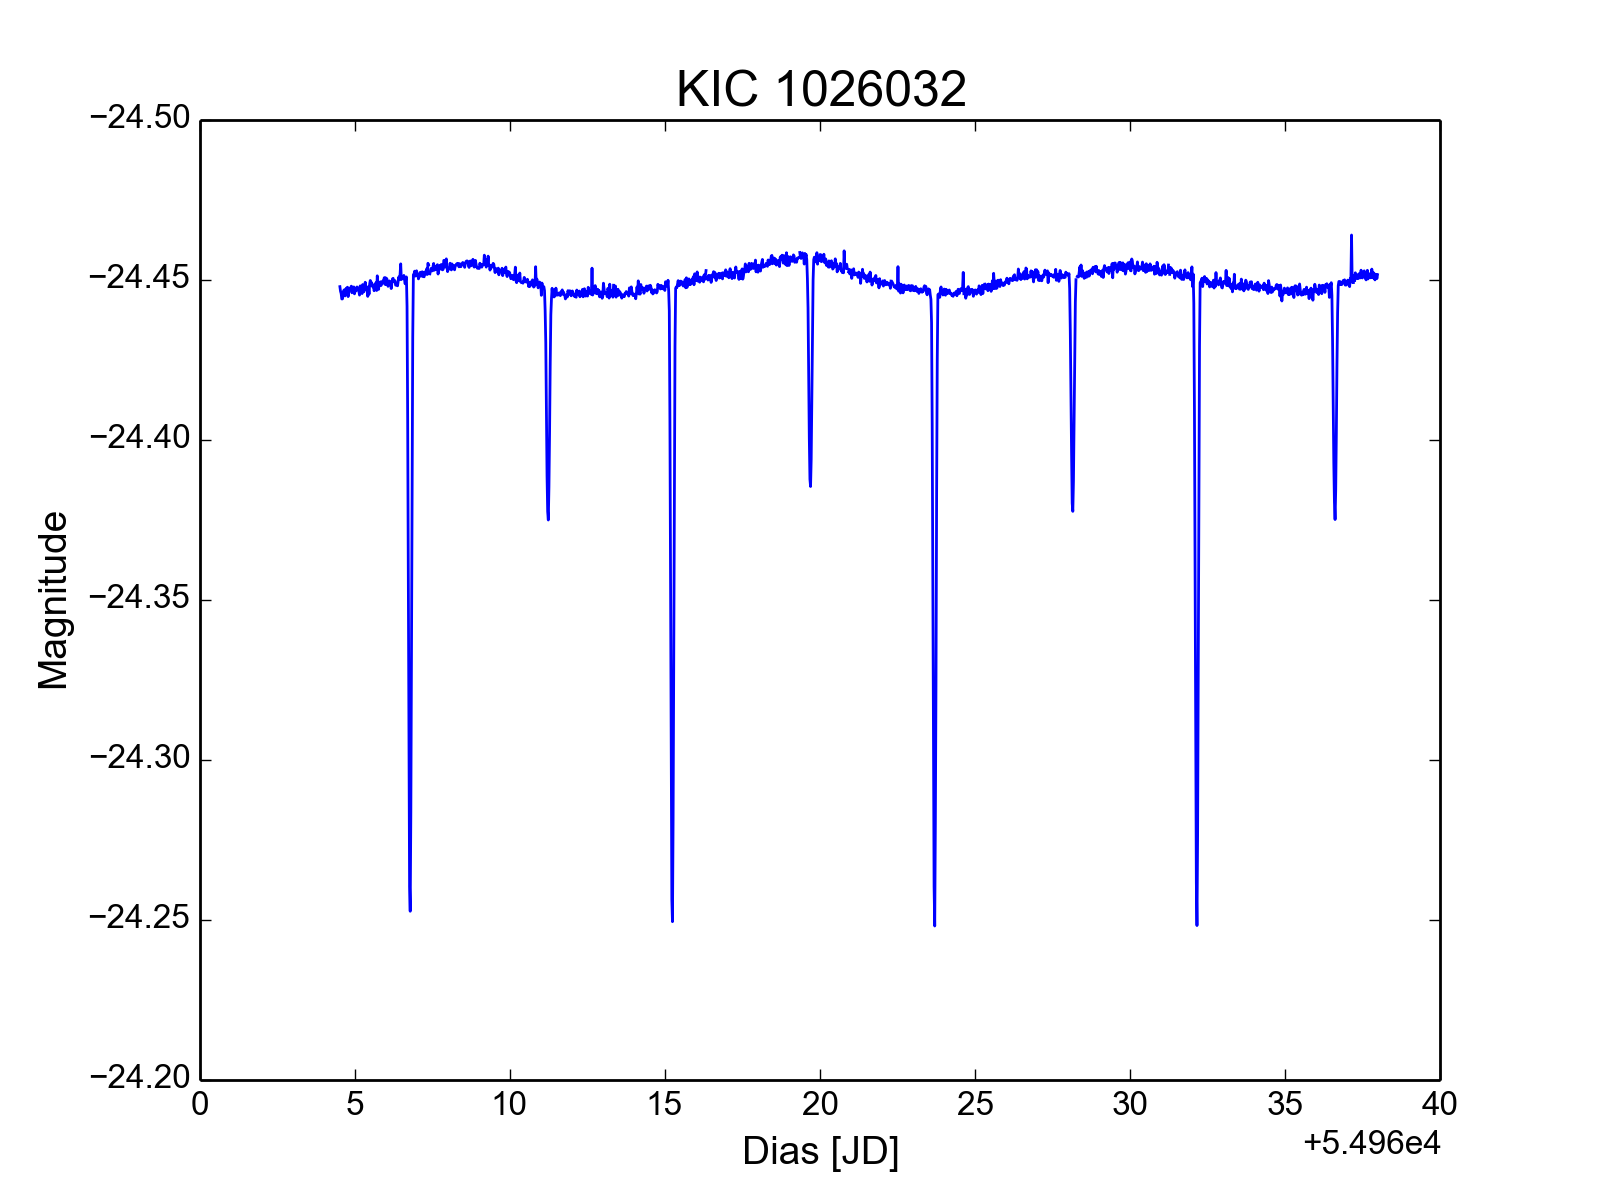
\includegraphics[width=\linewidth]{binary.png}
%   \caption{Sistema Binário}
%   \label{fig:binaria}
% \end{subfigure}%
% \begin{subfigure}{.5\textwidth}
%   \centering
%   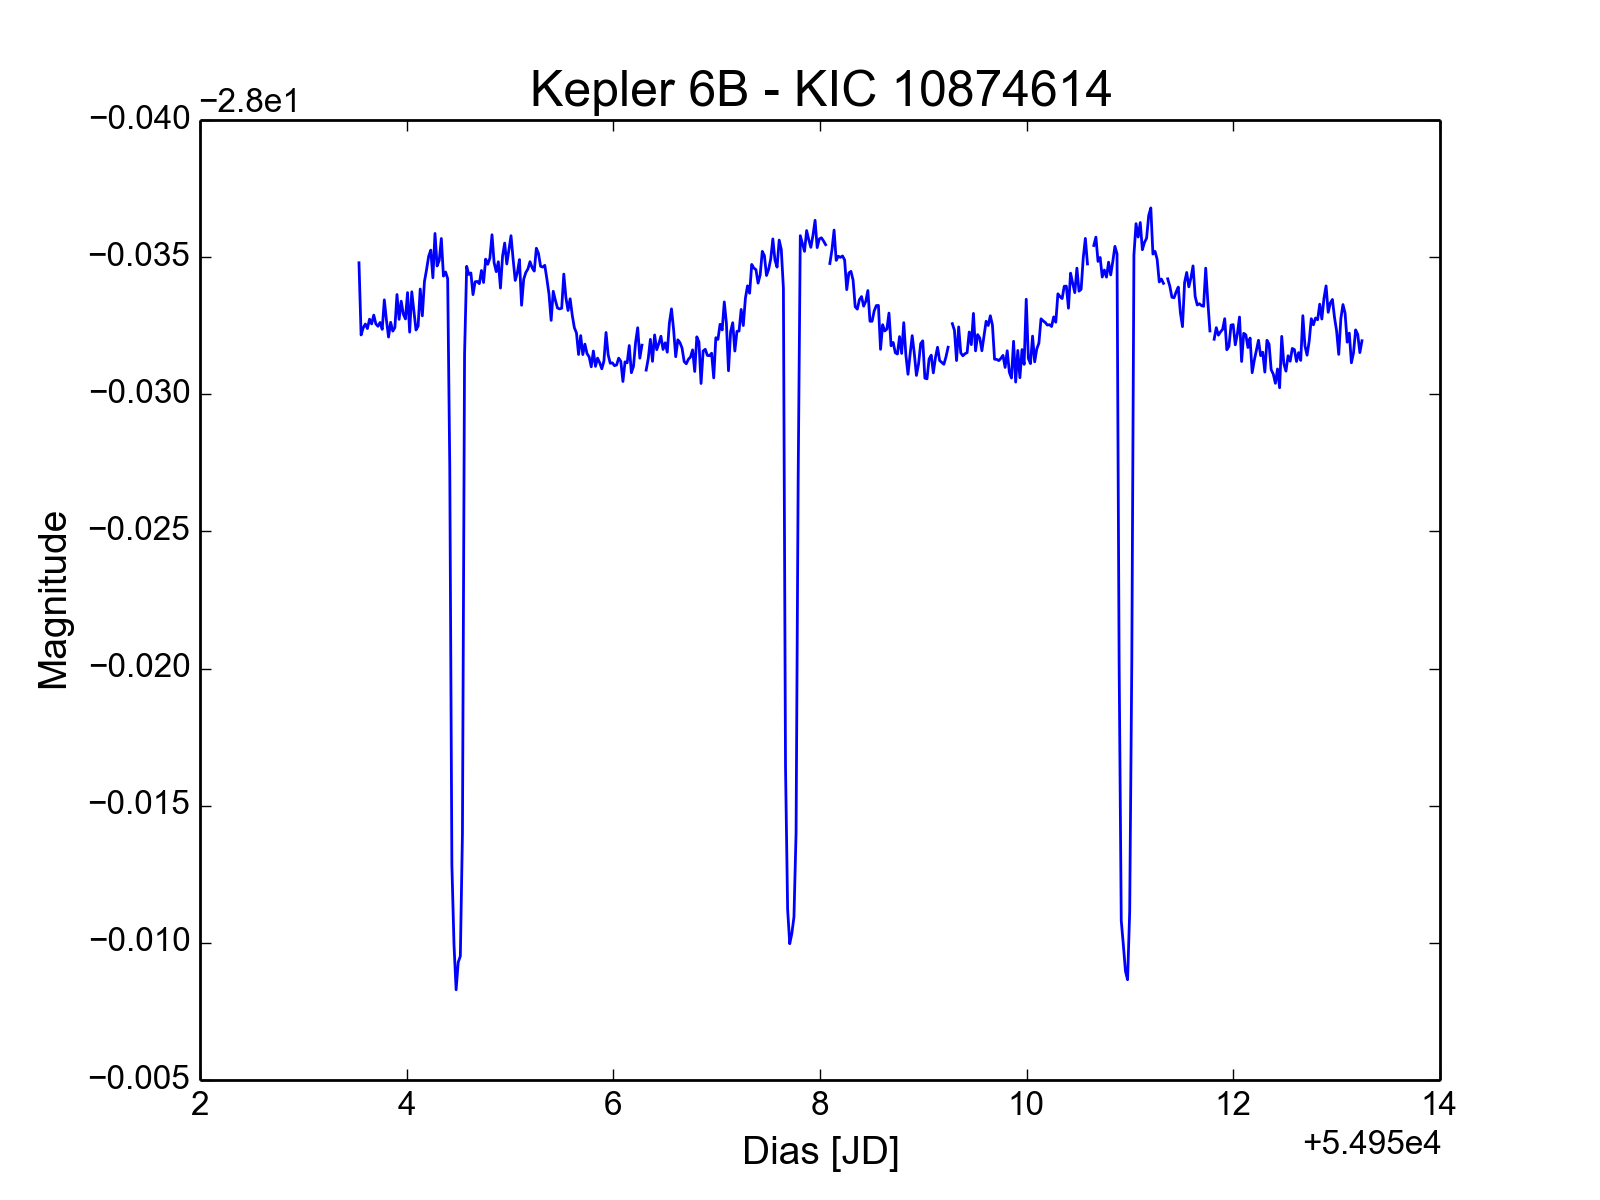
\includegraphics[width=\linewidth]{kepler6b.png}
%   \caption{Exoplaneta - Kepler 6B}
%   \label{fig:kepler6b}
% \end{subfigure}
% \caption{Exemplos de curvas de luz de variáveis eclipsantes para dados obtidos do Telescópio Kepler.}
% \label{fig:exemplo_eclipsantes}
% \end{figure}

% \end{frame}


\begin{frame}{Variáveis Intrínsecas}
O motivo da variação da magnitude está relacionada com processos internos da estrela
\begin{itemize}
    \item Eruptivas;
    \item Cataclísmicas;
    \item Pulsantes.
  \end{itemize}
\end{frame}

% \begin{frame}{Variáveis Intrínsecas - Eruptivas}
% \begin{itemize}
%   \item Estrelas em que ocorrem erupções na cromosfera e coroa
%   \item Essas erupções são chamadas de ventos solares
% \end{itemize}
% \end{frame}


% \begin{frame}[allowframebreaks]{Variáveis Intrínsecas - Cataclísmicas}
% \begin{itemize}
%   \item Divididas em \textit{Supernovas}, \textit{novas}, \textit{novas anãs} e \textit{simbióticas}
%   \item \textit{Novas} e \textit{novas anãs} são sistemas binários acretando matéria até o ponto em que o material acretado aquece o suficiente para queimar hidrogênio
%   \item \textit{Simbióticas} são semelhantes ao anterior porem ocorrendo em um periodo de tempo maior
% \end{itemize}

% \framebreak

% \begin{itemize}
%   \item \textit{Supernovas} são explosões com energias da ordem de $10^{45} \si{J}$ a $10^{47} \si{J}$.
% \end{itemize}

% \begin{figure}
% \centering
% 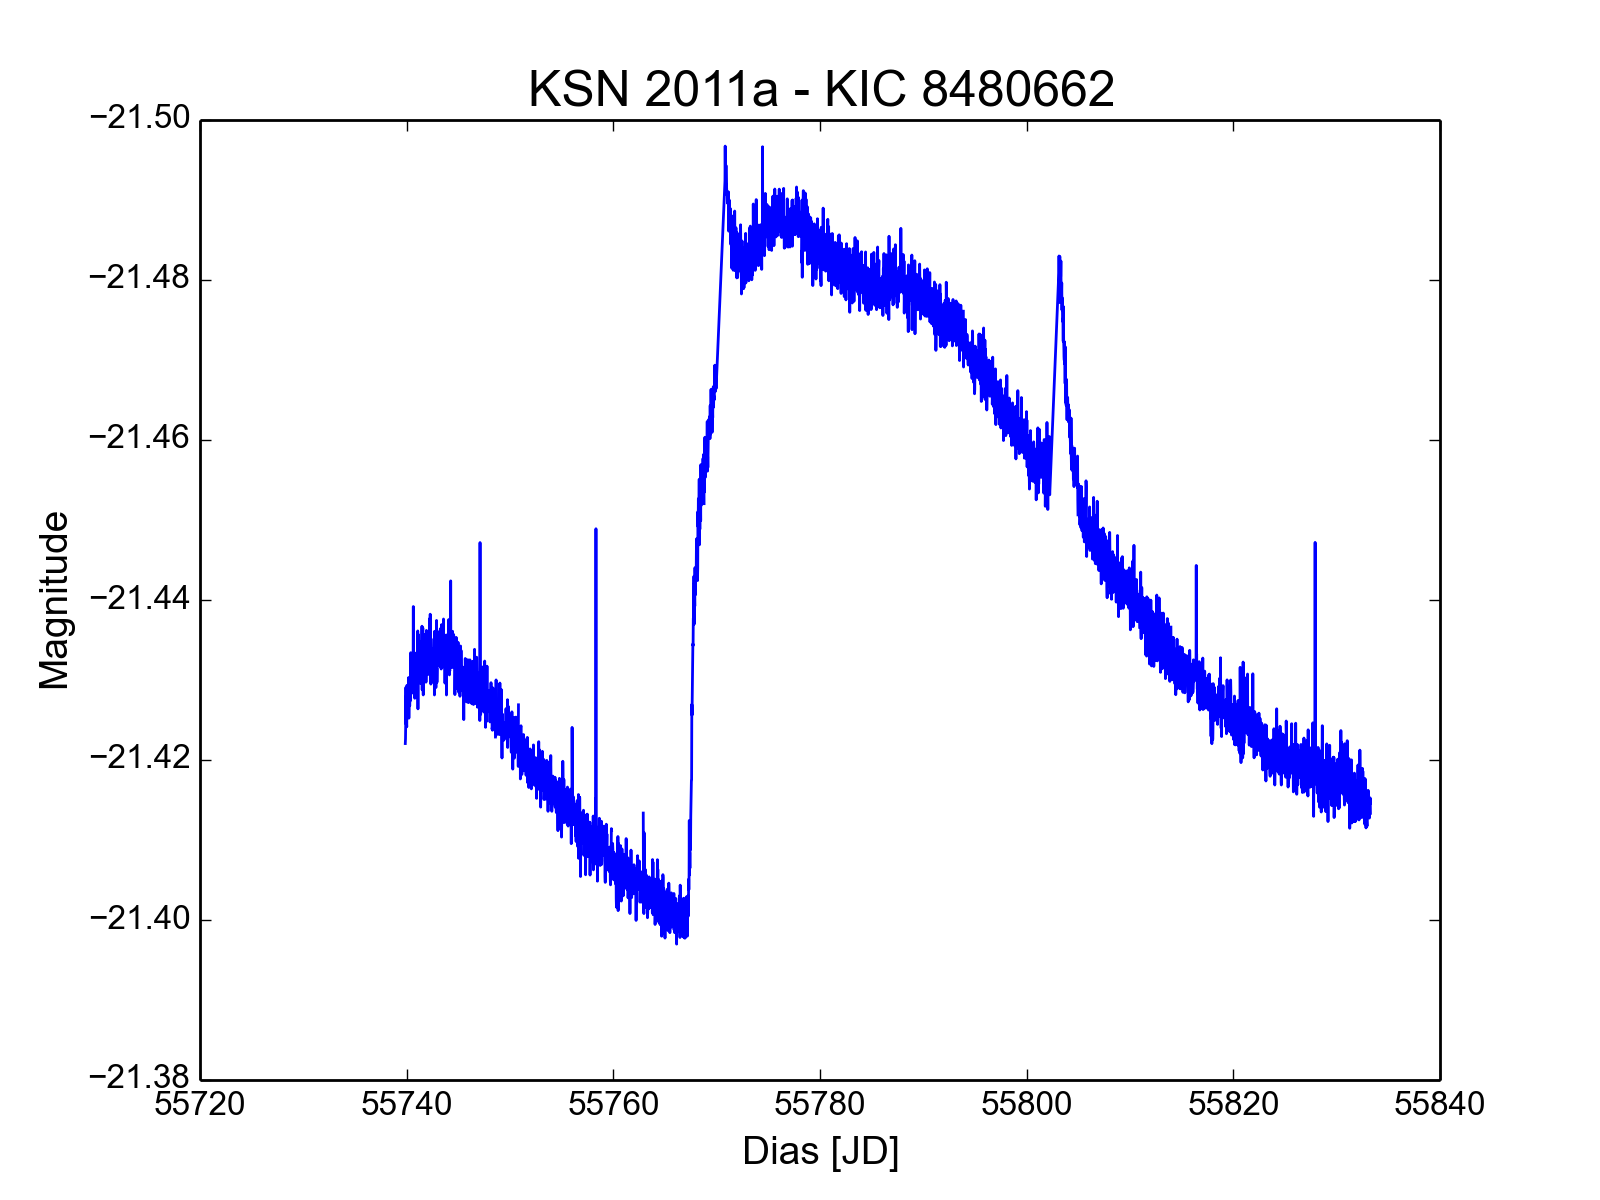
\includegraphics[width=0.5\linewidth]{sn2011a.png}
% \caption[Curva de luz da Supernova KSN 2011a]{Curva de luz da Supernova KSN 2011a observada pelo Telescópio Kepler em março de 2016.}
% \label{fig:exemplo_sn}
% \end{figure}
% \end{frame}

\begin{frame}{Variáveis Intrínsecas - Pulsantes}
\begin{itemize}
  \item Classe de estrelas que sofrem pulsações radiais
ou não-radiais ou até mesmo esses dois tipos de pulsação
  \item Exemplos:
  \begin{itemize}
    \item Cefeidas;
    \item RR Lyrae;
    \item Miras;
    \item Beta Cepheid;
    \item Gamma Doradus;
    \item etc.
  \end{itemize}
\item Objetos utilizados neste trabalho: \textit{Cefeidas} e \textit{RR Lyraes}.
\end{itemize}
\end{frame}

\begin{frame}[allowframebreaks]{Cefeidas Clássicas}
\begin{itemize}
   \item Estrelas que pulsam de forma radial;
   \item Podem possuir períodos entre 1 a 100 dias;
   \item Massa: $2$ M$_\odot$ a $20$ M$_\odot$
   \item População I (estrelas jovens, maior metalicidade)
   \item As cefeidas podem ser subdivididas de acordo com o seu modo de pulsação;
   \begin{itemize}
     \item FU: modo radial fundamental
     \item FO: primeiro sobre tom do modo radial
   \end{itemize}
 \end{itemize}

A grande importância deste tipo de estrela está na descoberta da relação entre
período e luminosidade derivada por Henrietta Leavitt \citep{Leavitt1912} o que possibilitou a determinação de distâncias estelares.

\framebreak

%################################################################################ COLOCAR A CURVA DE LUZ DE UMA CEFEIDA FU
%########################################################################
\begin{figure}
 \centering
  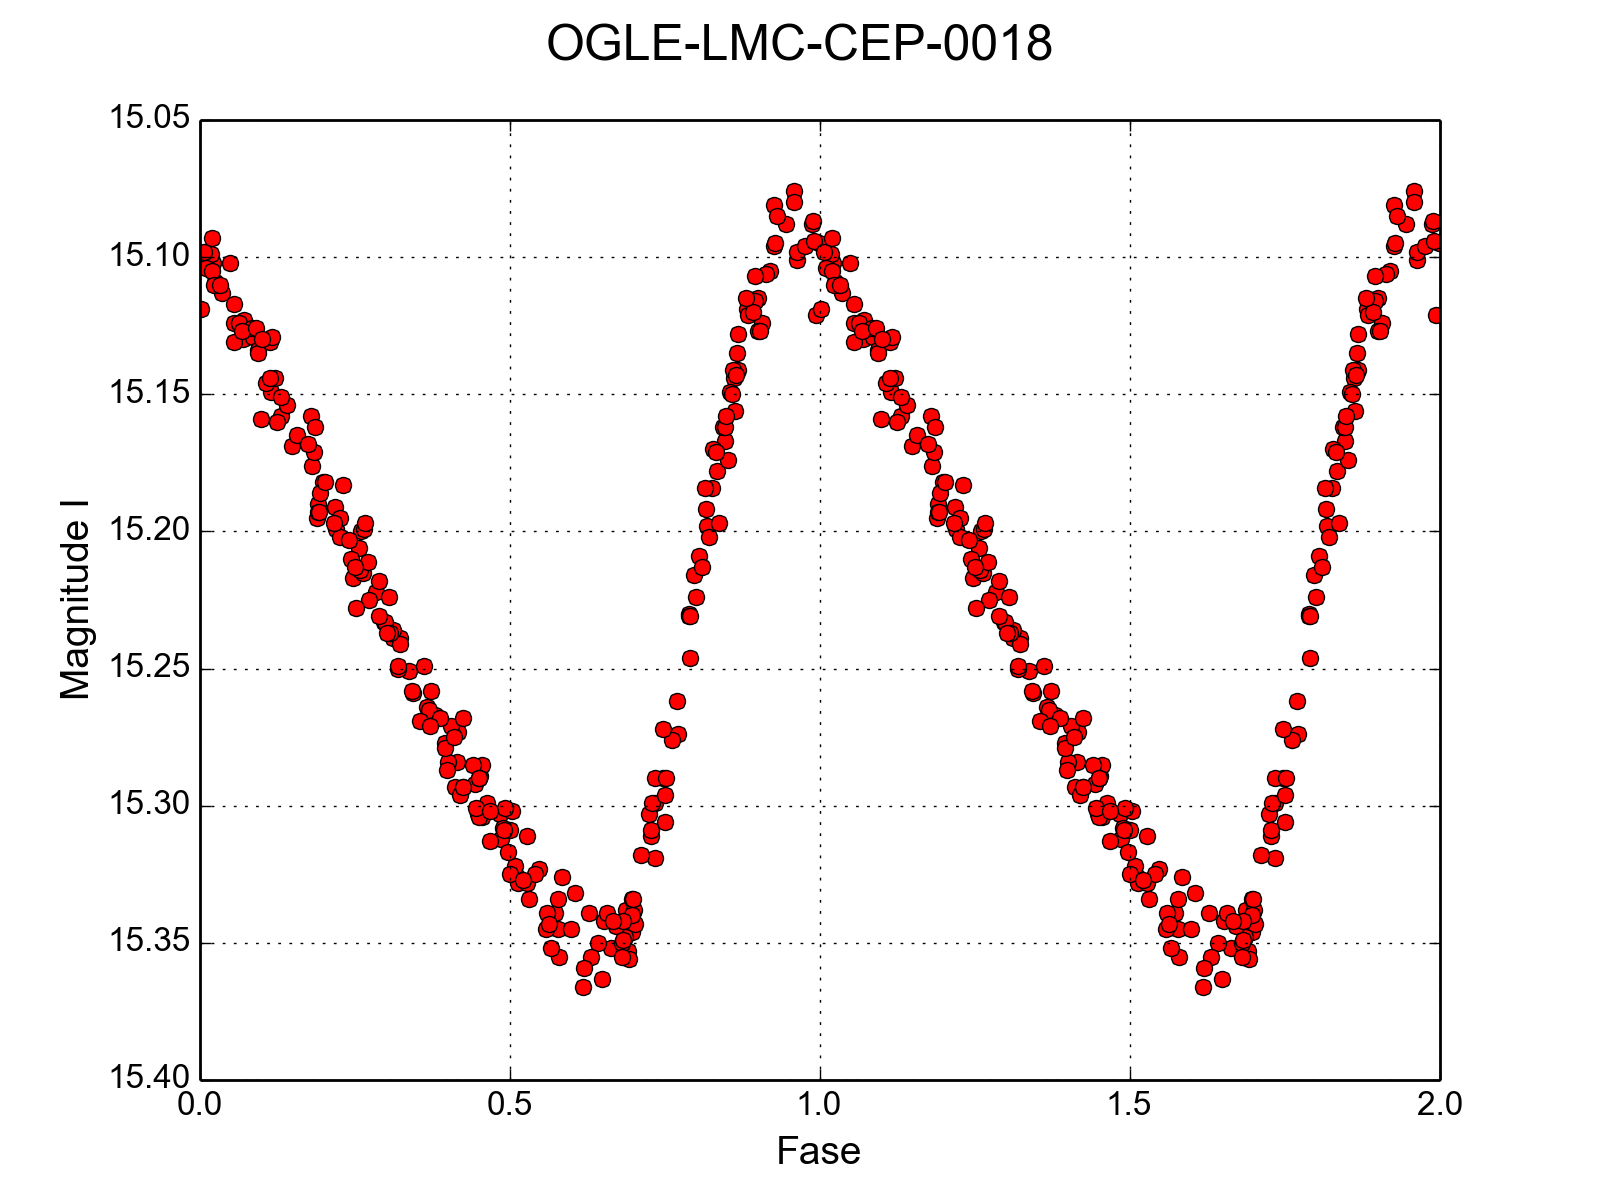
\includegraphics[width=0.68\linewidth]{0018_correct.png}
  \caption{Curva de luz no espaço de fase para uma Cefeida clássica ($P=4,0478$).}
  \label{fig:right}
\end{figure}
\end{frame}


\begin{frame}[allowframebreaks]{RR Lyrae}

\begin{itemize}
  \item Podem possuir períodos entre 0,2 a 1 dia;
  \item Massa: $0,6$ M$_\odot$ a $0,8$ M$_\odot$
  \item População II (estrelas antigas, menor metalicidade)
  \item Utilizadas para determinar distância de sistemas estelares antigos
  \item Classificas em AB (modo radial fundamental) e C (primeiro sobre-tom)
\end{itemize}

\framebreak

% \begin{figure}
% \centering
% \begin{subfigure}{.5\textwidth}
%   \centering
%   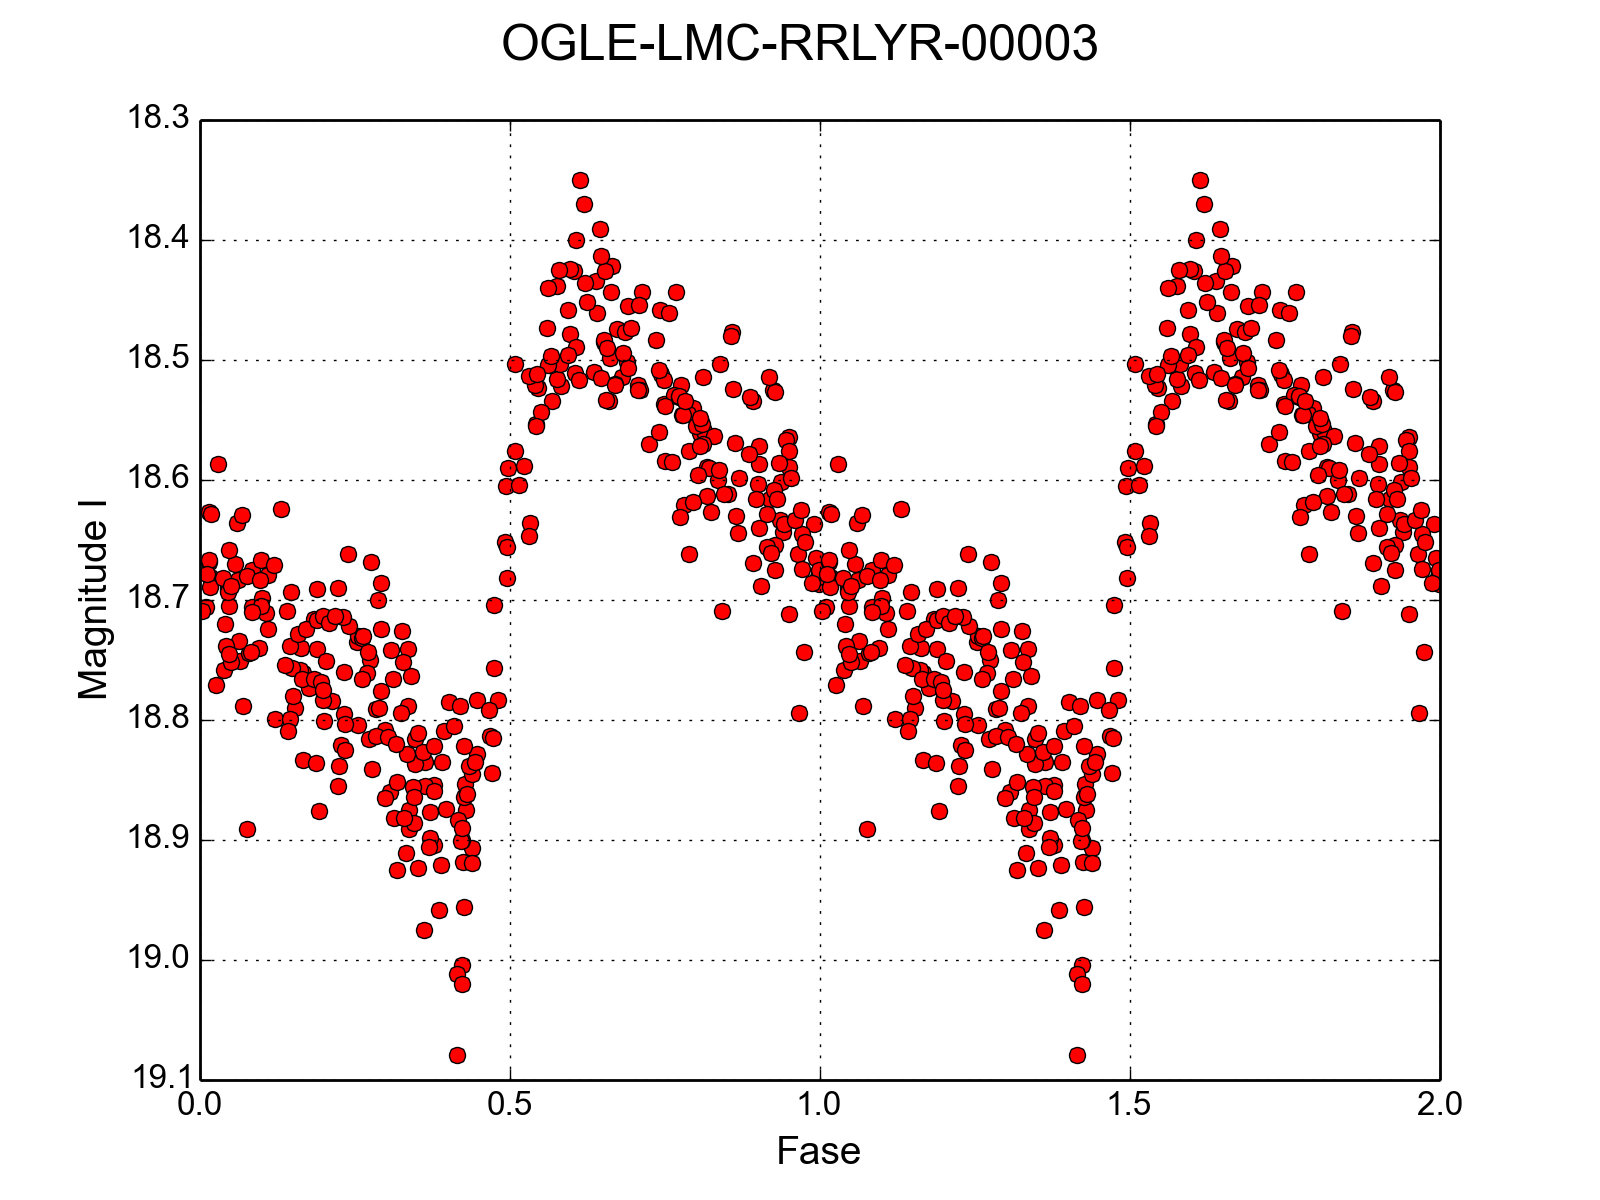
\includegraphics[width=\linewidth]{rrlyrAB.png}
%   \caption{RR Lyrae AB}
%   %\label{fig:right}
% \end{subfigure}%
% \begin{subfigure}{.5\textwidth}
%   \centering
%   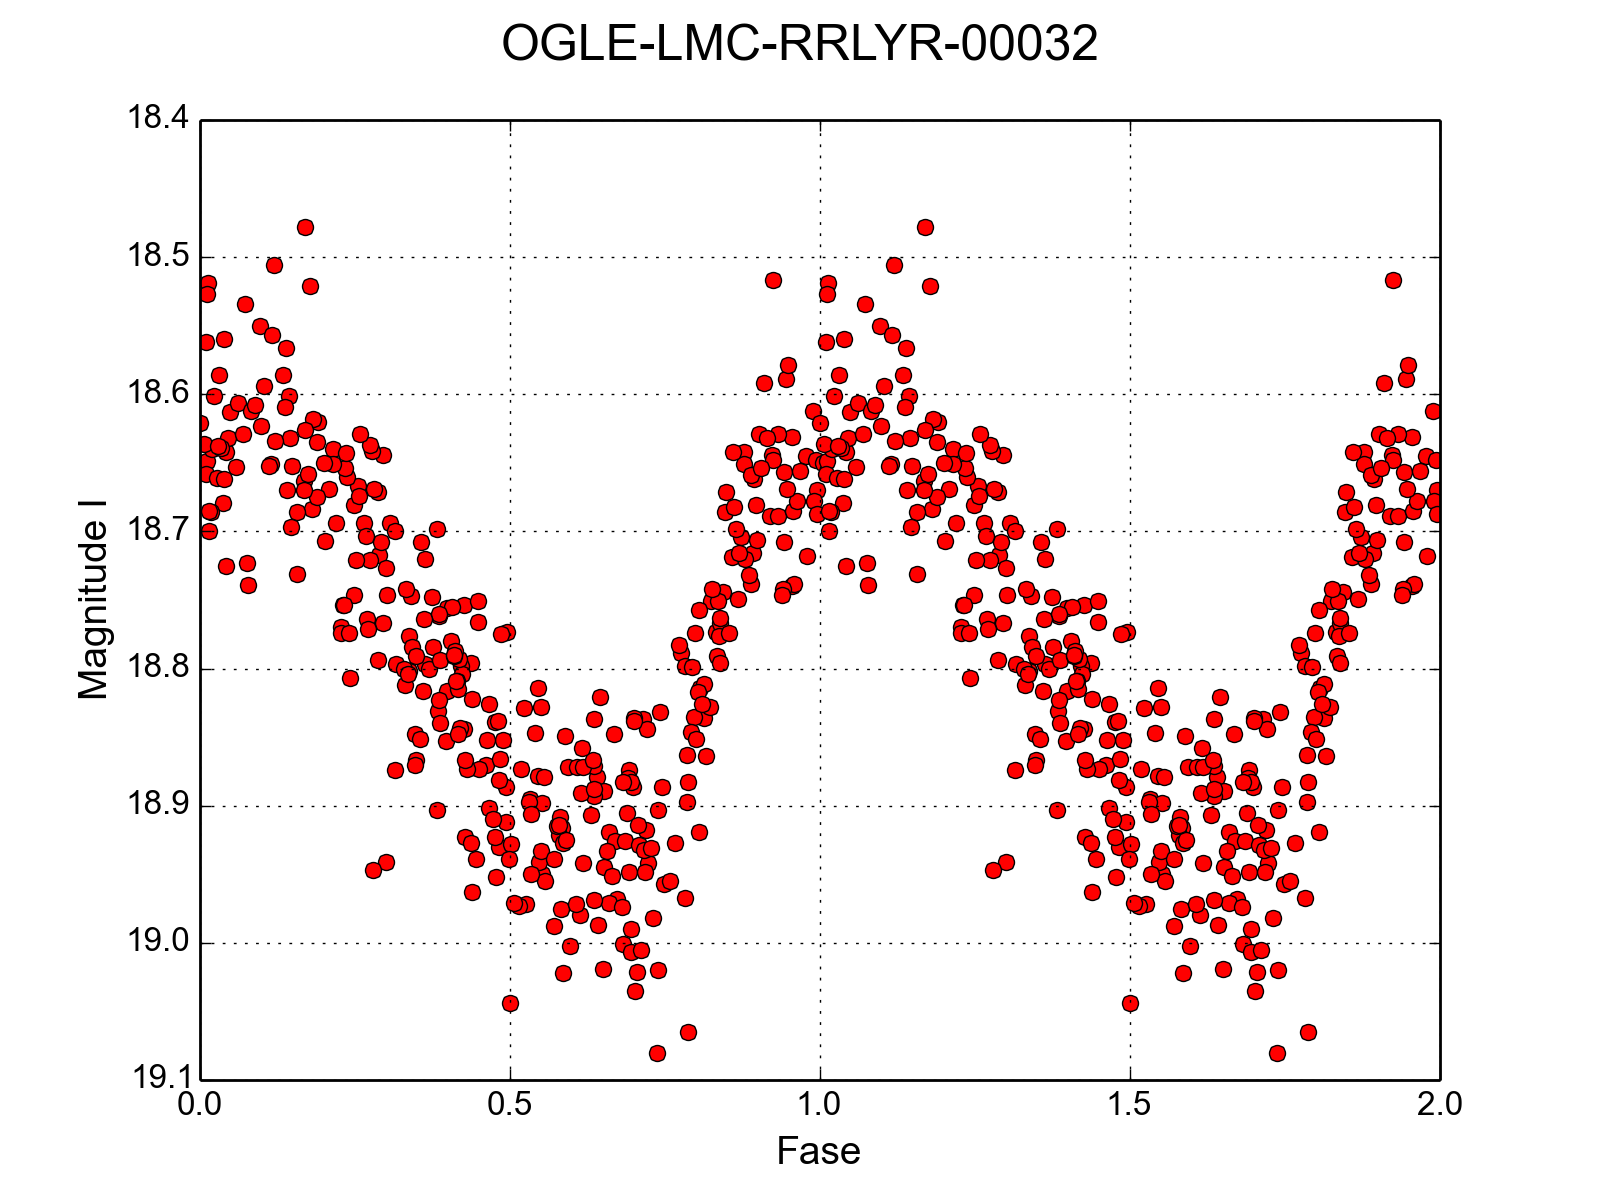
\includegraphics[width=\linewidth]{rrlyrC.png}
%   \caption{RR Lyrae C}
%   %\label{fig:wrong}
% \end{subfigure}
% \caption[Curva de luz de RR Lyrae]{Curvas de luz no espaço de fase para uma  RR Lyrae tipo $AB$ ($P=0,6565$) e uma tipo $C$ ($P=0,3535$) do catálogo OGLE.}
% \label{fig:exemplo_rrlyr}
% \end{figure}

\begin{figure}
\centering
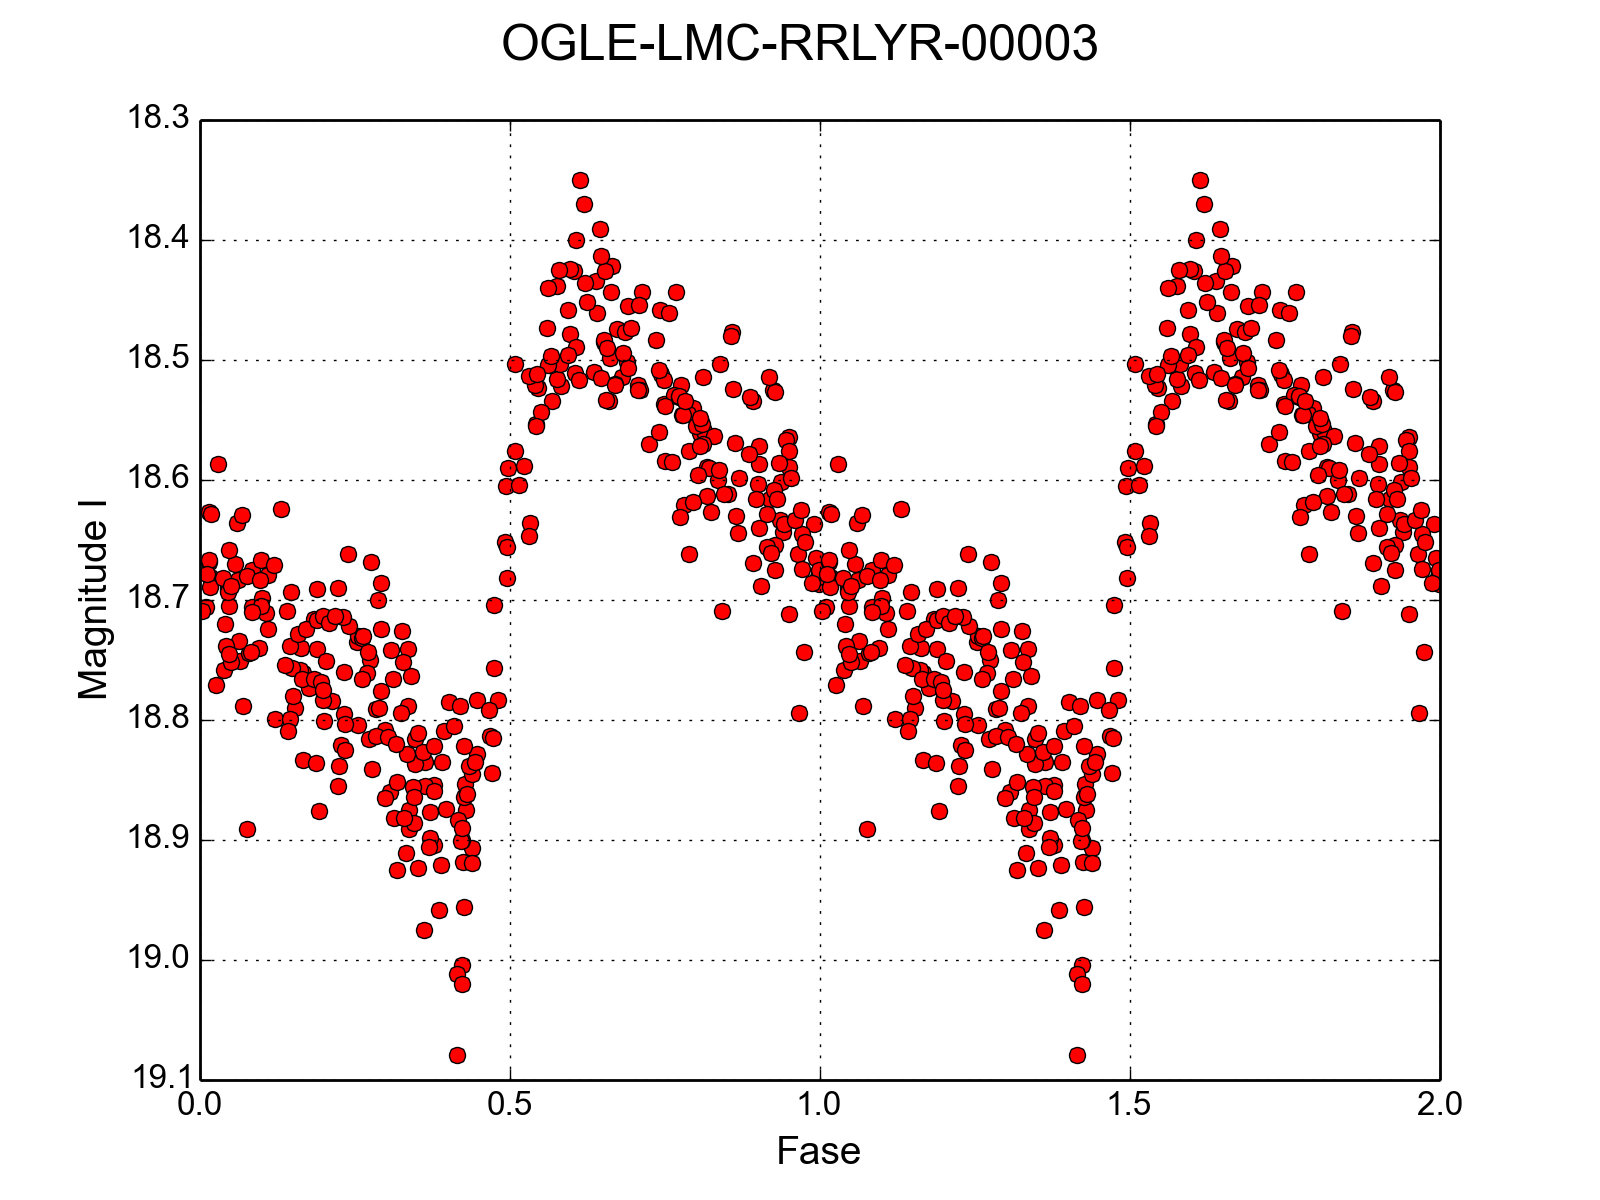
\includegraphics[width=0.68\linewidth]{rrlyrAB.png}
\caption{Curvas de luz no espaço de fase para uma  RR Lyrae tipo $AB$ ($P=0,6565$)}
\label{fig:right}
\end{figure}
\end{frame}


% \begin{frame}{Pulsação Estelar - Talvez}
%   talvez
% \end{frame}

\begin{frame}{Espaço de Fase}

\begin{itemize}
\item Estrela com comportamento periódico $\to$ ciclos iguais
\item Ciclo = Fase
\item Não importa qual ciclo estamos observando, apenas onde estamos no ciclo
\end{itemize}

O espaço de fase é uma representação de todos os ciclos observados em apenas uma fase, ou em apenas
um ciclo.
\vspace{5mm}

Os pontos de sobrepõem e formam uma oscilação geral da estrela. Este
espaço de fase é calculado pela seguinte expressão

\begin{equation}
\phi_i = \frac{t_i}{P} - \Big[\frac{t_i}{P}\Big]
\end{equation}


\end{frame}


% %-----------------------------------------------------------------------
% \section{Velas Padrões e Relação P-L}
% %-----------------------------------------------------------------------

% \begin{frame}{Velas Padrões e Relação P-L}
% %A grande importância das variáveis pulsantes está na determinação de distância.
% As variáveis pulsantes são utilizadas como \textit{Velas Padrões} para determinação de distâncias.

% \end{frame}

%-----------------------------------------------------------------------
\section{Entropia de Shannon}
%-----------------------------------------------------------------------

\begin{frame}[allowframebreaks]{Entropia de Shannon}

\begin{itemize}
  \item Na teoria de informação, a entropia ou entropia de Shannon \citep{informationTheory} é a medida de incerteza de uma variável;
  \item Essa grandeza mede o grau de desordem de um sinal.
\end{itemize}

Aplicado para curvas de luz:
\begin{itemize}
  \item Curva de luz $\to$ Sinal periódico;
  \item Transformando para o espaço de fase
  \begin{itemize}
    \item Período correto: Espaço de fase possui ordem
    \item Período incorreto: Espaço de fase desordenado
      \end{itemize}
\end{itemize}

\framebreak

Fazendo $m$ repartições no espaço de fase, a entropia é definida por:
\begin{align}
H = - \sum_i^m \mu_i \ln \mu_i
\end{align}
em que $\mu_i$ representa a probabilidade de ocupação da repartição $i$.
\framebreak

\begin{figure}
\centering
\begin{subfigure}{.5\textwidth}
  \centering
  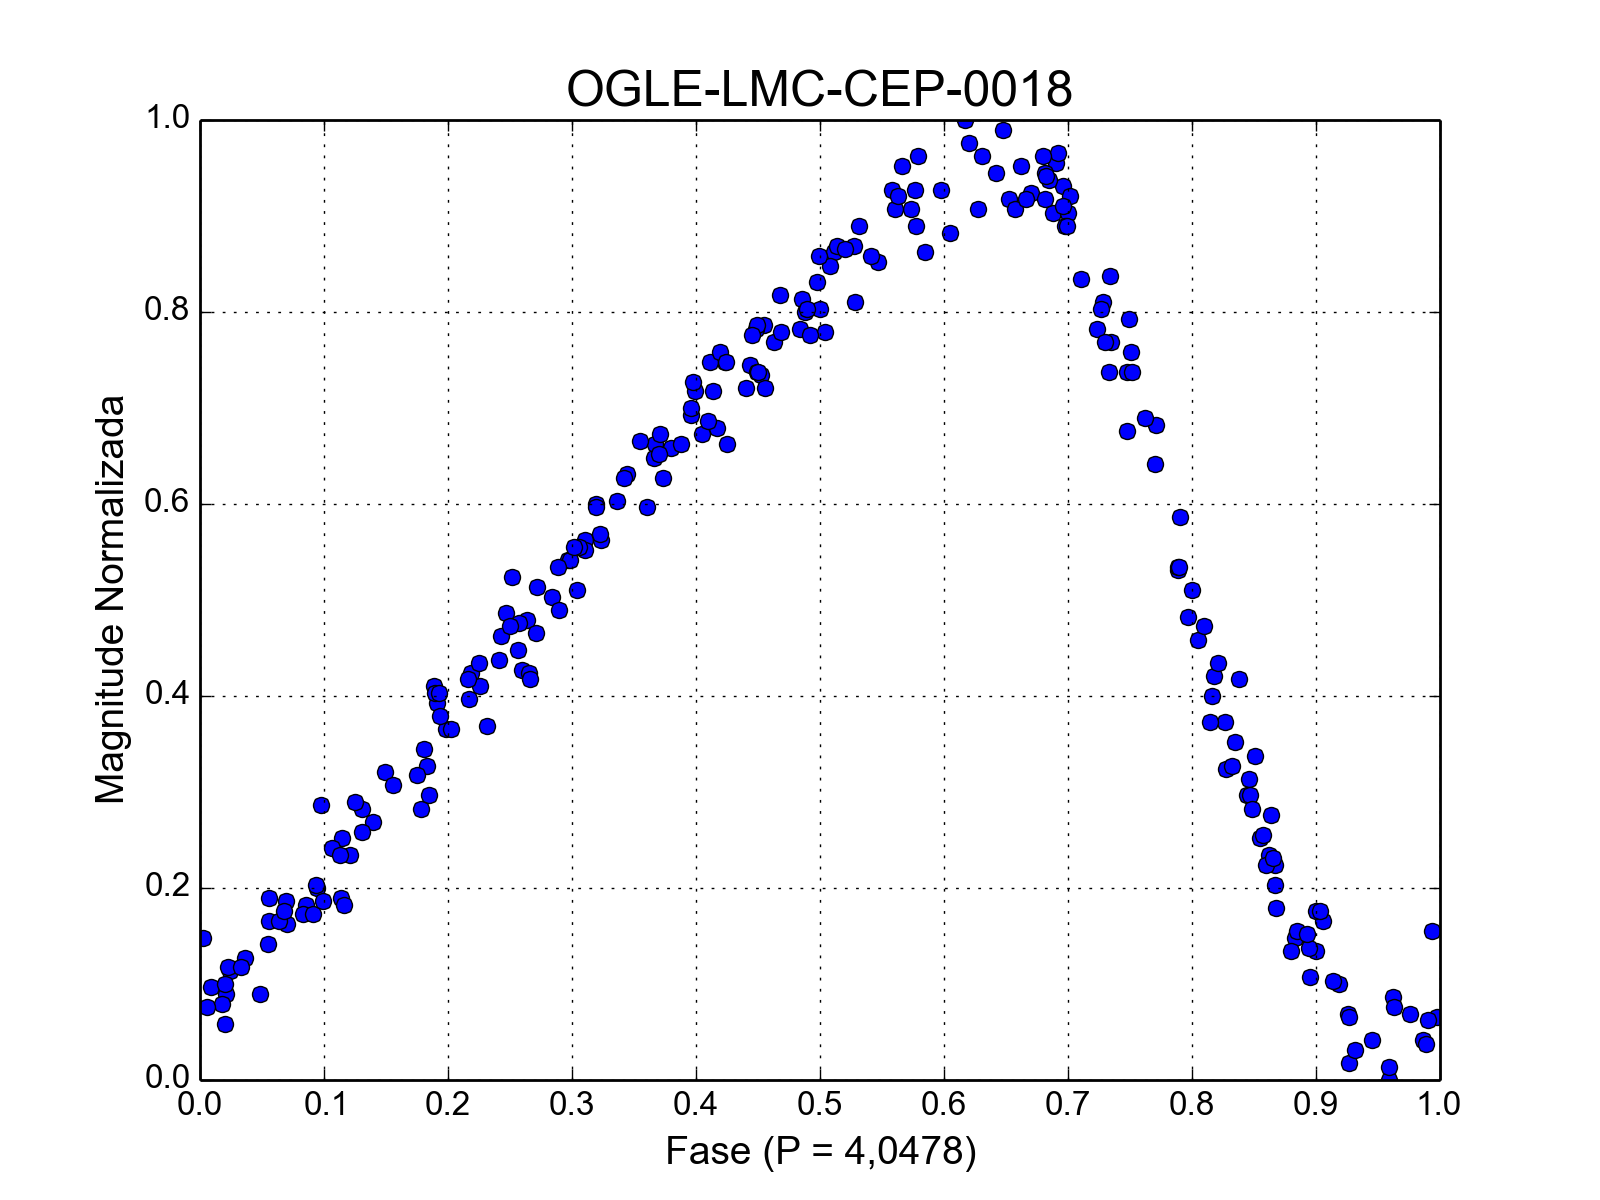
\includegraphics[width=\linewidth]{esp_fase_correto.png}
  \caption{Período correto, $H_c = 1,0762$}
  \label{fig:esp_fase_correto}
\end{subfigure}%
\begin{subfigure}{.5\textwidth}
  \centering
  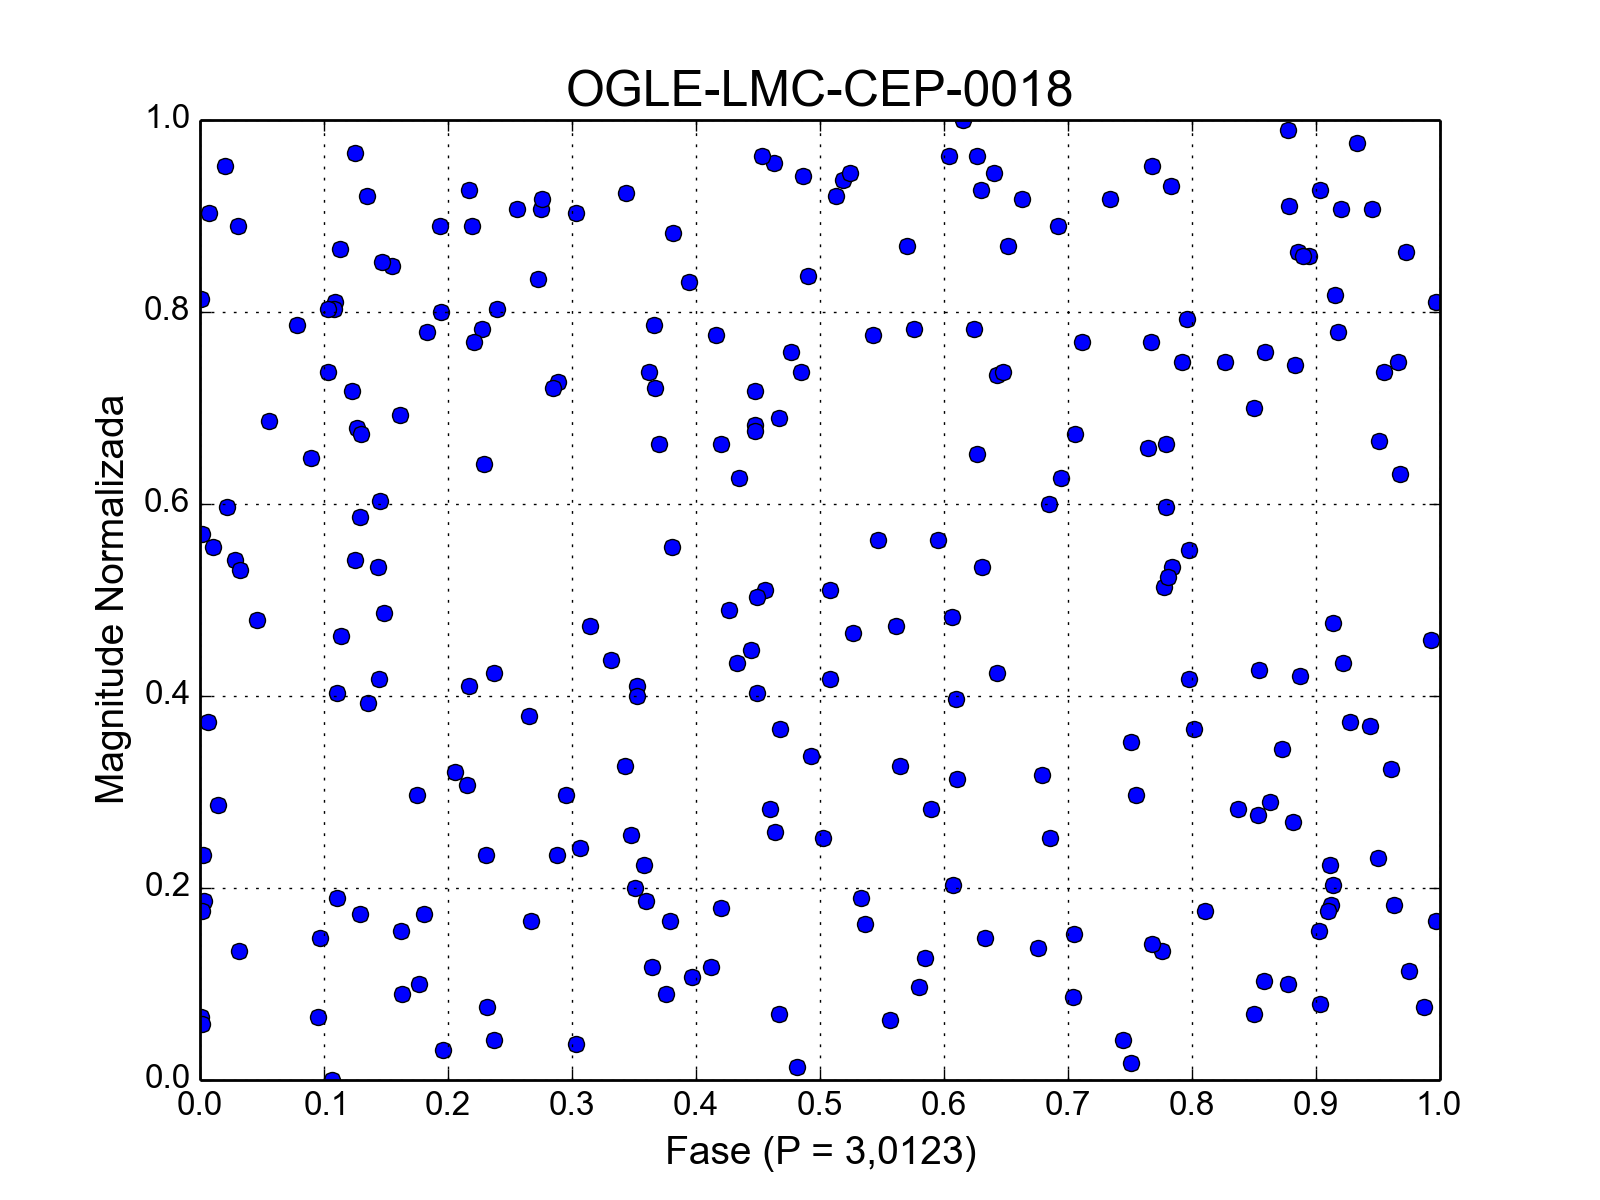
\includegraphics[width=\linewidth]{esp_fase_errado.png}
  \caption{Período errado, $H_c = 1,5943$}
  \label{fig:esp_fase_errado}
\end{subfigure}
\caption[Exemplos de entropia]{Exemplos da distribuição de pontos espaço de fase para a Cefeida OGLE-LMC-CEP-0018 do catálogo OGLE.}
\label{fig:exemplo_entropia}
\end{figure}
\end{frame}


\begin{frame}[allowframebreaks]{Entropia de Shannon Condicional}
A entropia de Shannon condicional surgiu da necessidade de contornar um
problema bem conhecido da analise de curvas de luz:
\begin{itemize}
  \item Erro no periodo $P=1$ dia
\end{itemize}

Devido as observações serem efetuadas durante a noite ocasionando um espaçamento de um dia entre os conjuntos de pontos.

\framebreak

\begin{figure}
\centering
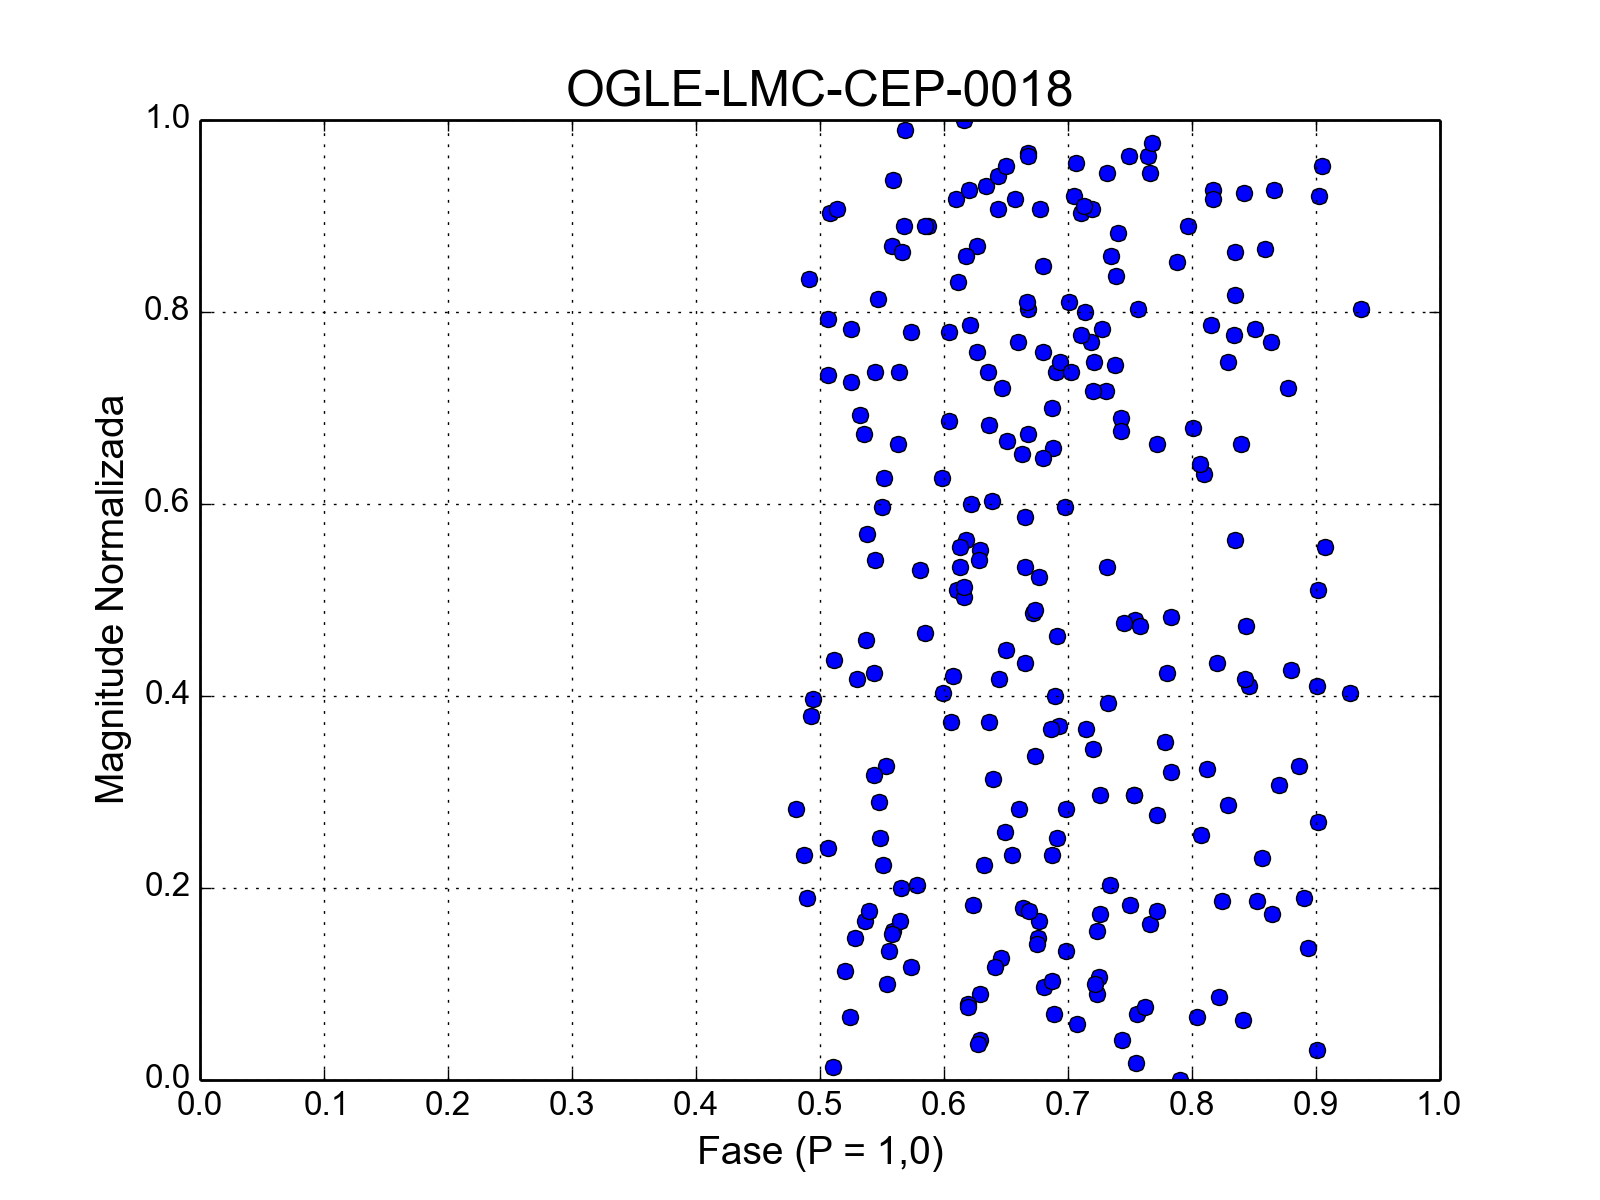
\includegraphics[width=0.65\linewidth]{esp_fase_1dia.png}
\caption{Efeito de \textit{Aliasing} devido ao período de 1 dia para a Cefeida OGLE-LMC-CEP-0018 do catálogo OGLE. $H_c=1,5542$.}
\label{fig:periodo1dia}
\end{figure}

\framebreak

Para lidar com esse problema, \citet{ce} propuseram a entropia de Shannon condicional.

\begin{itemize}
  \item O espaço de fase é dividido em $i$ repartições na magnitude e $j$ repartições na fase
  \item Entropia é calculada da seguinte forma:
\end{itemize}
\begin{align}
H_c = \sum_{i,j} p(m_i,\phi_j) \ln \left( \frac{p(\phi_j)}{p(m_i,\phi_j)} \right)
\end{align}
em que $p(m_i,\phi_j)$ é a probabilidade de ocupação na $i$-ésima repartição da magnitude e na $j$-ésima repartição da fase e $p(\phi_j)$ é a probabilidade de ocupação na $j$-ésima repartição da fase.
\framebreak

\begin{figure}
\centering
\begin{subfigure}{.5\textwidth}
  \centering
  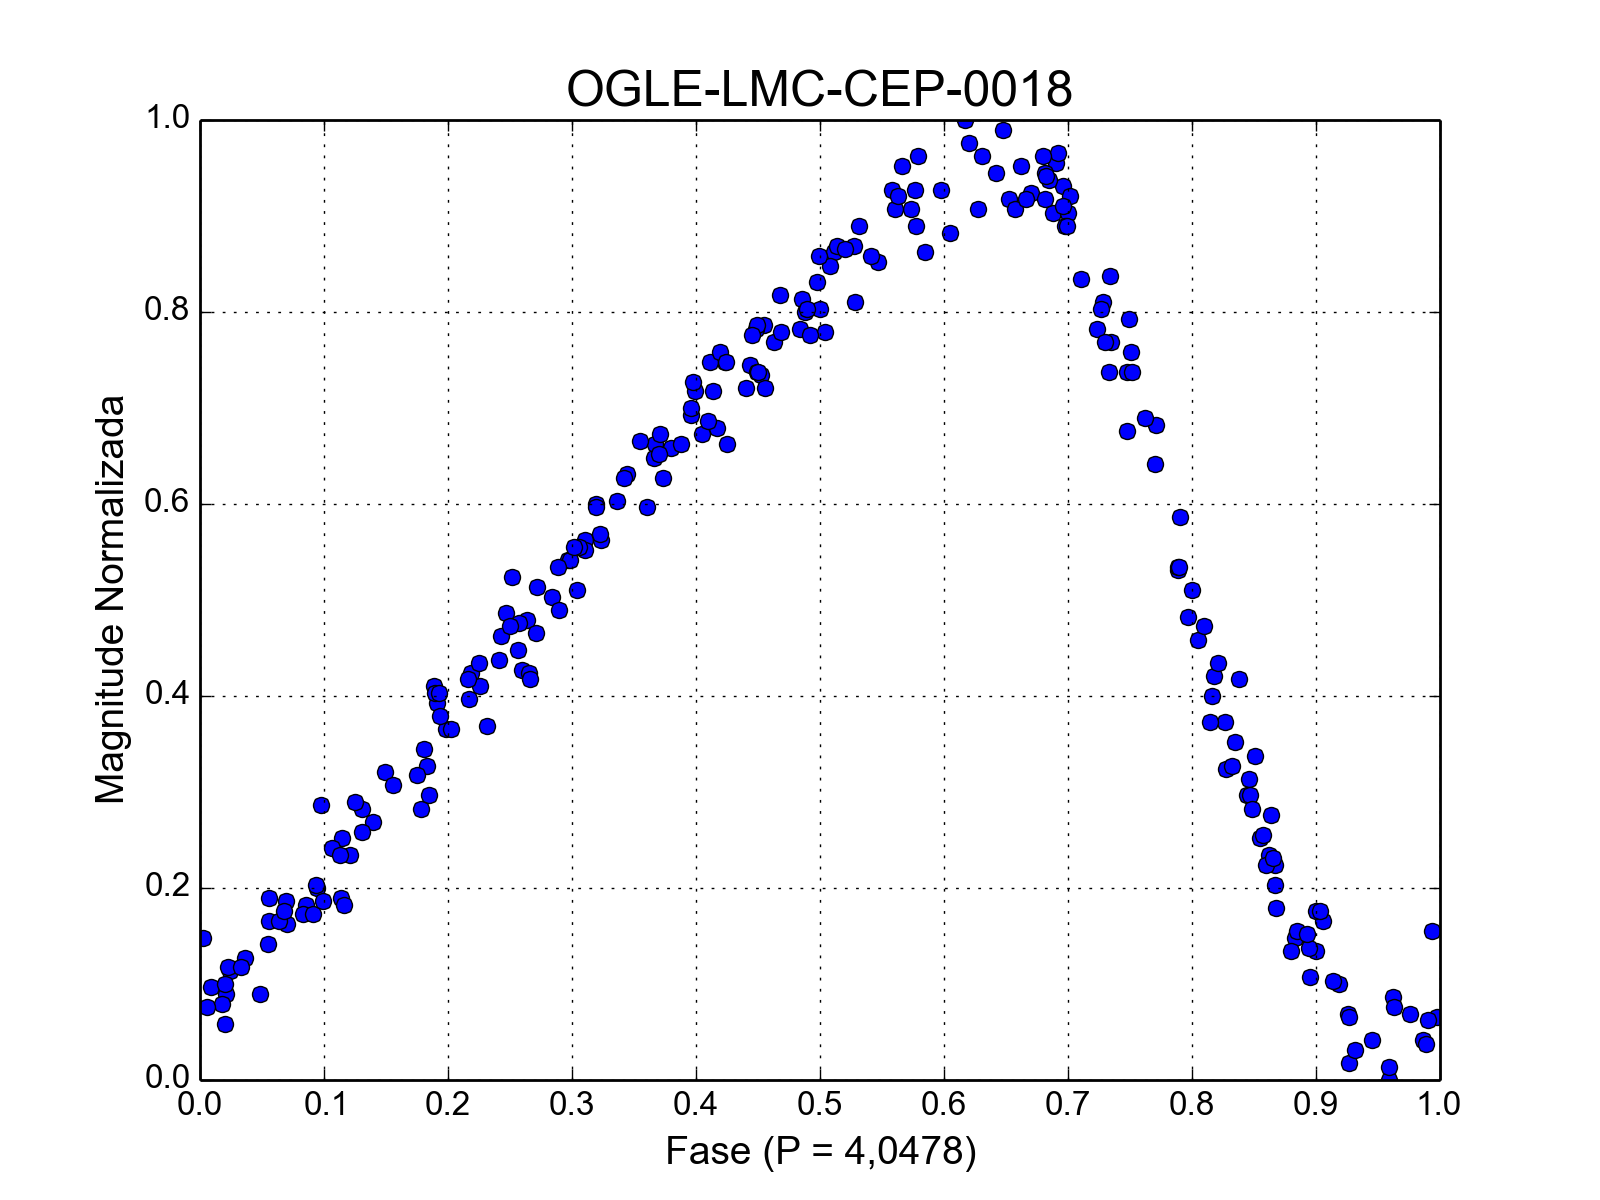
\includegraphics[width=\linewidth]{esp_fase_correto.png}
  \caption{Período correto, $H_c = 1,0762$}
  \label{fig:esp_fase_correto2}
\end{subfigure}%
\begin{subfigure}{.5\textwidth}
  \centering
  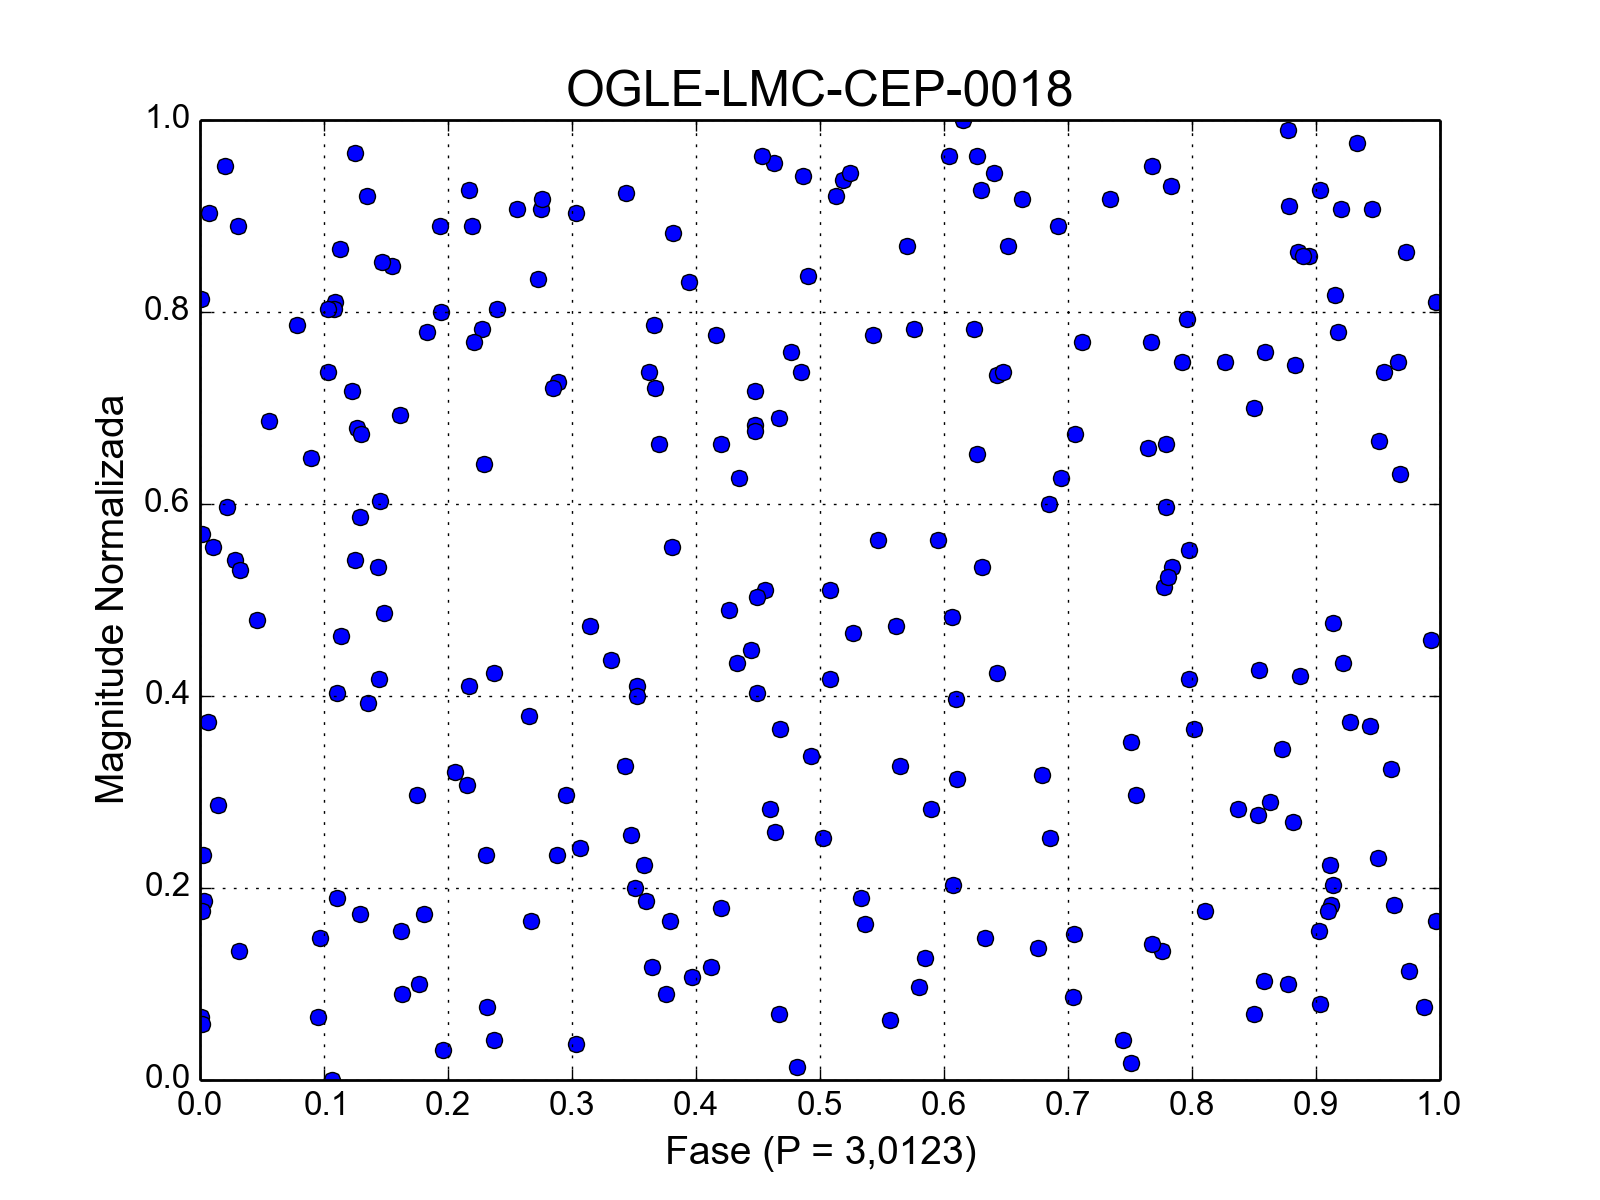
\includegraphics[width=\linewidth]{esp_fase_errado.png}
  \caption{Período errado, $H_c = 1,5943$}
  \label{fig:esp_fase_errado2}
\end{subfigure}
\caption[Exemplos de entropia]{Exemplos da distribuição de pontos espaço de fase para a Cefeida OGLE-LMC-CEP-0018 do catálogo OGLE.}
\label{fig:exemplo_entropia2}
\end{figure}

\end{frame}

%-----------------------------------------------------------------------
\section{Algoritmo}
%-----------------------------------------------------------------------

\begin{frame}{Algoritmo}

Foi desenvolvido um algoritmo em \texttt{Python3} para calcular a entropia condicional. O algoritmo funciona da seguinte maneira:

\vspace{.1cm}
\begin{block}{Para cada estrela:}
%\textbf{Para cada estrela:}
  \begin{itemize}
    \item Os dados tempo e magnitude são lidos como vetores
    \item Um vetor com períodos é criado
    \item O espaço de fase é criado para cada período
    \item A entropia da dispersão no espaço de fase é calculado
    \item A menor entropia de todos os períodos é identificada
    \item O período associado a esta entropia é escolhido como o correto
  \end{itemize}
\end{block}


\end{frame}


%-----------------------------------------------------------------------
\section{Catálogo OGLE e Resultados}
%-----------------------------------------------------------------------


\begin{frame}{Dados do Catálogo OGLE}
Algoritmo aplicado para dados do Catálogo OGLE (\textit{The Optical Gravitational Lensing Experiment}) \citep{Udalski2008}

\begin{itemize}
  \item 8 anos de dados observacionais;
  \item Área de 40 graus quadrados na direção das Nuvens de Magalhães;
  \item Busca por estrelas variáveis;
  \item Banda I e V
  \item Os dados são públicos
\end{itemize}

\end{frame}

\begin{frame}{Resultados - OGLE}
Foram analisadas um total de $25707$ estrelas variáveis do Catálogo OGLE.
\begin{table}
\begin{center}
\caption{Quantidade de dados analisados e resultados corretos considerando uma precisão de $10^{-4}$.}
\begin{tabular}{c|c|c|c}
\hline
Estrelas & Quantidade & Acertos  & Porcentagem \\
\hline
Cefeidas FU & $1818$ & $1817$ & $99,94 \%$ \\
Cefeidas FO & $1238$ & $1231$ & $99,43 \%$ \\
%\hline
RRLyraes AB& $17693$ & $17540$ & $99,14 \%$ \\
RRLyraes C& $4958$ & $4535$ & $91,47 \%$ \\
\hline
\textbf{Total} & $\textbf{25707}$ & $\textbf{25123}$ & $\textbf{97,73 \%}$ \\
\hline
\end{tabular}
\label{tab:resultados}
\end{center}
\end{table}

\end{frame}

%-----------------------------------------------------------------------
\section{Análise Teórica e Resultados}
%-----------------------------------------------------------------------

\begin{frame}[allowframebreaks]{Análise Teórica}

A fim de entender como os dados afetam no resultado do método, foi analisado o comportamento da entropia de Shannon para dados com diferentes níveis de ruído e pontos.

\begin{itemize}
\item Utilizando os dados das RRLyraes como referência, foram obtidos as grandezas:
\begin{itemize}
\item \(t_i = 2152.5019\) HJD,
\item \(t_f = 4539.4593\) HJD,
\item quantidade de pontos \(n \approx 351\)
\item \(dt = \frac{t_f - t_i}{n}\)
\item Amostragem: $f_s = \dfrac{1}{dt} =  0.1473$ Hz
\end{itemize}
\end{itemize}

\framebreak

Possuindo a amostragem média dos dados observacionais, podemos construir dados sintéticos variando a amostragem e o ruido.

\begin{block}

De acordo com \cite{ce} e \cite{entropy}, para construir dados sintéticos semelhantes com os dados observacionais da maioria dos Surveys de estrelas variáveis, podemos utilizar a seguinte expressão,
\begin{align}
m(t) &= A_0 + \sum_i^3 A_n \sin \Big( \frac{2 n \pi t}{P} \Big) + \varepsilon \eta \label{eq:sinal}
\end{align}
\end{block}
em que \(\varepsilon\) é um fator de escala para o ruido entre \(0.0\) e \(1.0\), \(\eta\) é uma distribuição gaussiana com média zero e desvio unitário. \(P\) é o período médio das RRlyraes que, segundo \cite{lyraes} é de \(0.576\) dias.


\framebreak

% \begin{itemize}
% \item A influencia da amostragem está no vetor \(t\) que é construindo a fim de representar de forma mais fiel possível os dados do Catálogo OGLE-III.
% \begin{itemize}
% \item  \(dt = \frac{1}{f}\)
% \item \(f = n \times f_s\)
% \item \(n\) é um parâmetro de escala para a amostragem.
% \end{itemize}
% \item O ruído é controlado pelo fator \(\varepsilon\) na equação \eqref{eq:sinal}
% \end{itemize}
% \end{frame}

% \begin{frame}{Dados Sintéticos}

\begin{itemize}
  \item Foram gerados dados sintéticos variando:
  \begin{itemize}
    \item Amostragem: variando de $0.25$ a $4$ com intervalo de $0.25$
    \item Ruído: $\varepsilon$ de $0.0$ até $1.0$ com intervalo de $0.05$
  \end{itemize}
  \item Total de $300$ curvas de luz.
\end{itemize}

\end{frame}

\begin{frame}%{Resultados - Análise Teórica}
 \begin{figure}
\centering
\hspace{-1.cm}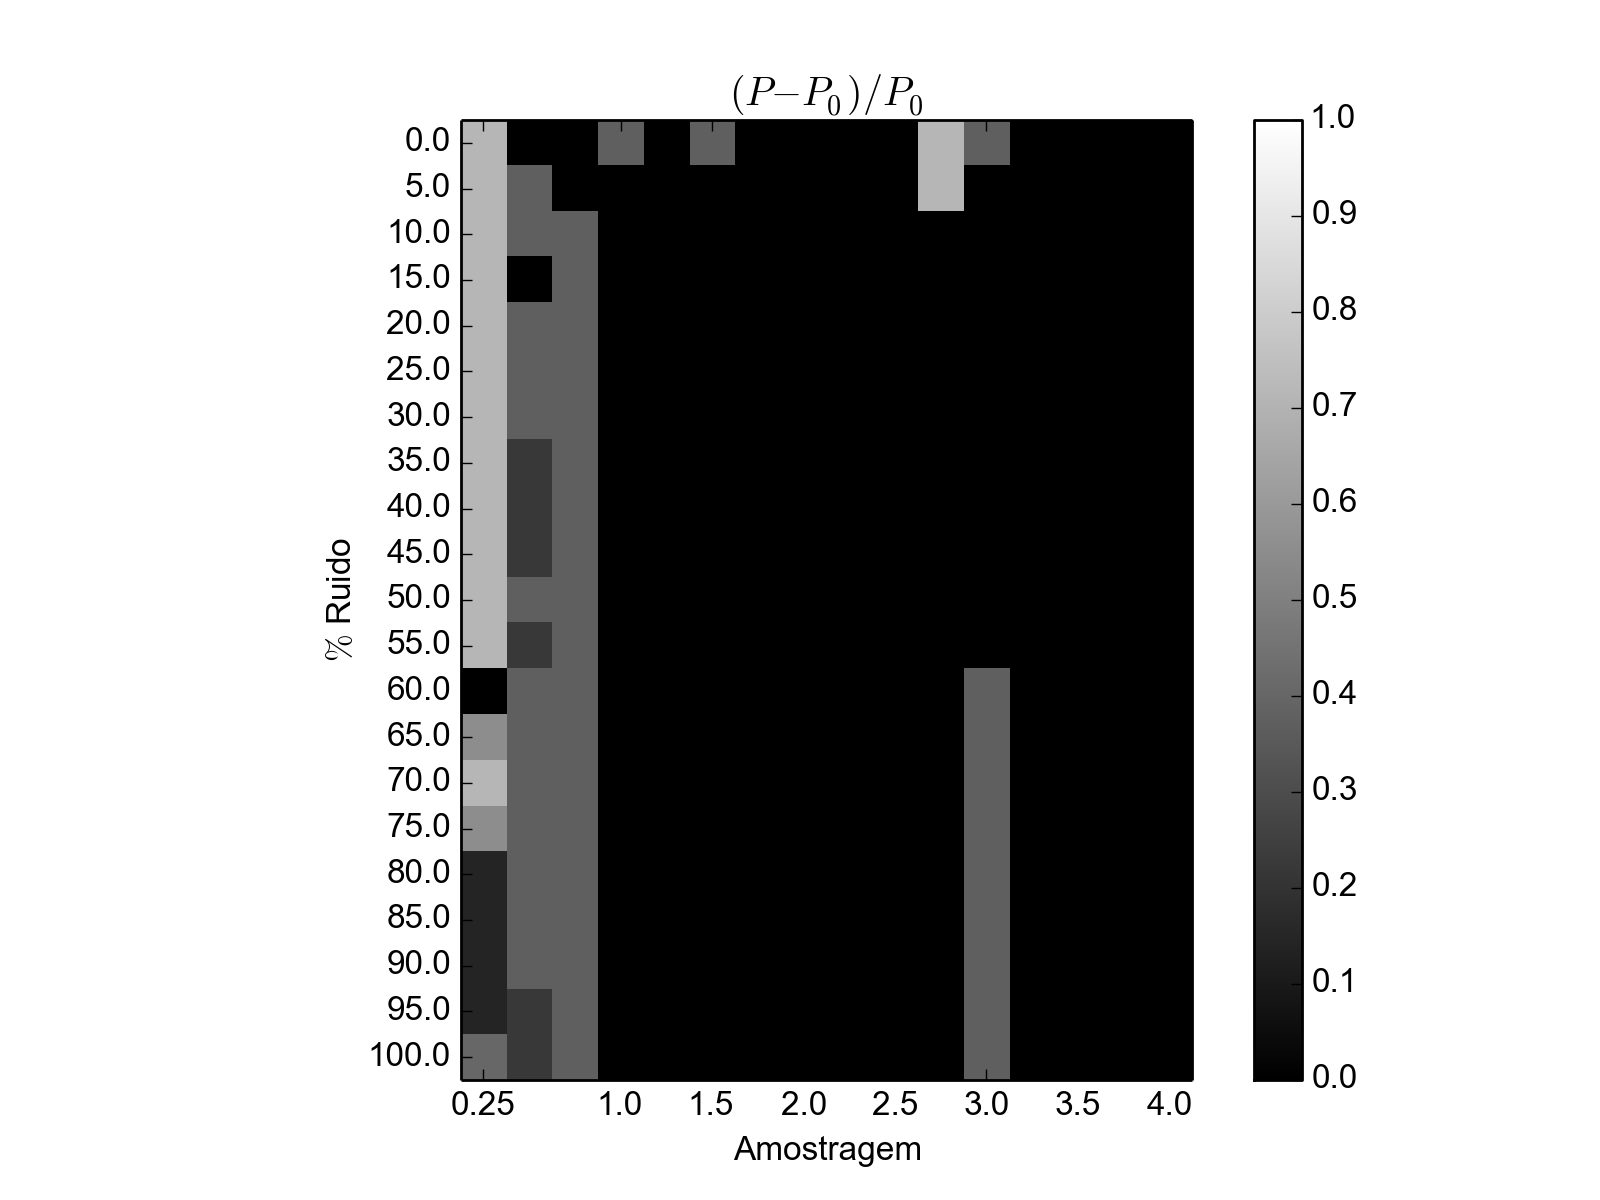
\includegraphics[scale=.5]{ce_inshow.png}
\label{fig:imshow}
\caption{Resultados obtidos em escala de cinza}
\end{figure}
\end{frame}

%-----------------------------------------------------------------------
\section{Aplicação}
%-----------------------------------------------------------------------

\begin{frame}[allowframebreaks]{Aplicação dos Resultados}
A grande importância da determinação de períodos de estrelas variáveis está na possibilidade de calcular distâncias a partir da Lei de Leavitt. Utilizando essa relação,
\begin{align}
\bar{M_i} = a \log P_i + b
\end{align}
e o modulo de distância $\mu = m - M - A_\lambda$ obtemos
\begin{align}
\bar{m_i} = a \log P_i + b + \mu_i + A_{\lambda_i} \label{eq:cap4_pl}
\end{align}

é possível calcular as constantes $a$ e $b$ utilizando o método dos mínimos quadrados.
A extinção interestelar $A_\lambda$ é dada pelo mapa de \citet{Pejcha2009}

\framebreak

\begin{table}[ht]
\begin{center}
\caption{Constantes da Relação PL.}
\begin{tabular}{c|c|c}
\hline
Objeto & $a$ & $b^\prime$ \\
\hline
Cefeida FU & $-1,292$ & $16,878$ \\
Cefeida FO & $-1,573$  & $16,558$ \\
RR Lyrae AB & $-0,721$ & $18,363$\\
RR Lyrae C & $-0,022$ & $18,841$\\
\hline
\end{tabular} \\
\label{tab:pl_relacao}
\end{center}
\end{table}

\framebreak

Obtendo essas relações, é possível calcular a variação na distância $\Delta \mu_i$ de cada uma das estrelas pelo residual entre a Lei de Leavitt e a magnitude média obtida pelos dados do catálogo, ou seja,
\begin{align}
\Delta \mu_i = \bar{m}_{OGLE} - \bar{m_i}
\end{align}
considerando uma distância média de $50\si{kpc}$ ou $\bar{\mu} = 18,495$ \citep{Pejcha2009}.

\framebreak
Para calcular a distribuição das estrelas é necessário fazer uma transformação de coordenadas, passando de ($\alpha$, $\delta$, $r$) para ($x$, $y$, $z$)
As transformações de coordenadas são dadas por \citet{Deb2014} e mostradas a seguir:
\begin{align}
x &= -r \sin \left(\alpha - \alpha_0 \right) \cos \left( \delta \right) \notag \\
y &= r \sin \left( \delta \right) \cos \left( \delta_0 \right) - r \sin \left( \delta_0 \right) \cos \left( \alpha - \alpha_0 \right) \cos \left( \delta \right) \label{eq:cap4_trans}\\
z &= r_0 - r \sin \left( \delta \right) \sin \left(\delta_0 \right) - r \cos \left( \delta_0 \right) \cos \left( \alpha \right) - \alpha_0 \cos \left( \delta \right) \notag
\end{align}

O centro da Grande Nuvem de Magalhães é obtido a partir dos valores médios das coordenadas equatoriais $\alpha$ e $\delta$ e possui valores $\alpha_0 = 80,240^\circ$ e $\delta_0 = -69.608^\circ$.

\framebreak

\begin{figure}
\centering
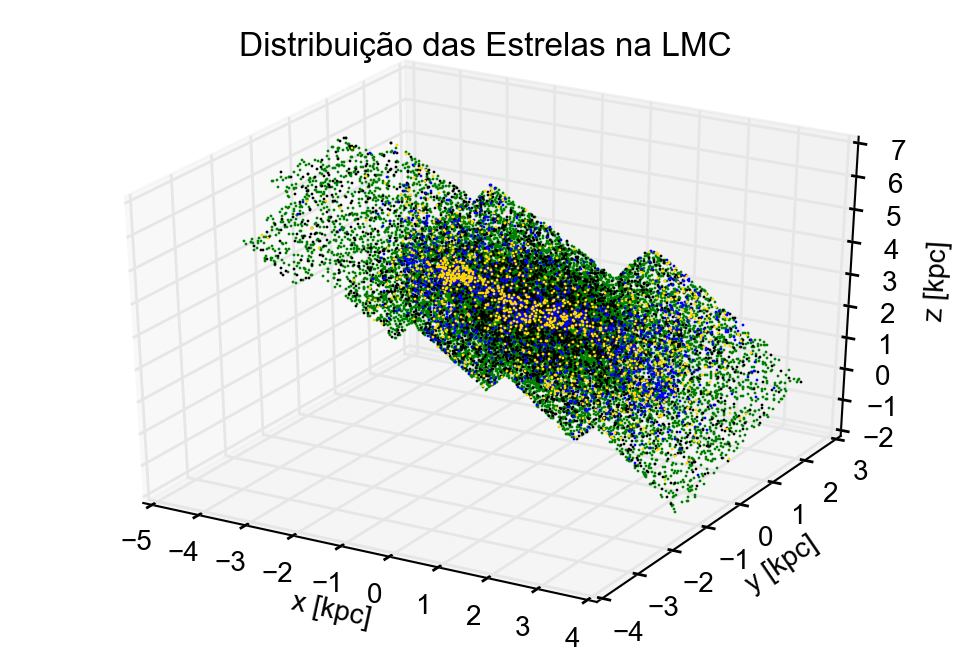
\includegraphics[width=0.8\linewidth]{plot3d.png}
\caption{Distruição 3D das variáveis pulsantes na LMC.}
\end{figure}
\end{frame}

%-----------------------------------------------------------------------
\section{Conclusão}
%-----------------------------------------------------------------------

\begin{frame}{Conclusão}

\begin{block}{Entropia de Shannon Condicional}

\begin{itemize}
  \item Técnica simples de ser aplicada;
  \item Embasada na Teoria da Informação
  \item Taxa de acerto maior do que $97\%$
\end{itemize}
\end{block}


\begin{block}{Analise dos dados sintéticos}
\begin{itemize}
  \item O método é confiável para qualquer nível de ruído desde que a frequência de pontos dos dados seja maior do que $f_s = 0,1473$.
  \item Ferramenta que nos indica como os dados influenciam no resultado do método
  \item É Possível determinar como a observação nos telescópios devem ser conduzidas
\end{itemize}
\end{block}

\end{frame}

%-----------------------------------------------------------------------
\section{Referências}
%-----------------------------------------------------------------------

\begin{frame}[allowframebreaks]{Referências}
%\nocite{*}
\footnotesize
\bibliography{ref}
\end{frame}


\begin{frame}

   \centering
    \LARGE{Obrigado!} \\
    \vspace{4mm}
    \normalsize{Perguntas?}

\end{frame}


% \begin{frame}{Dados Sintéticos}
% \begin{itemize}
% \item A fim de entender como os dados afetam no resultado do método, vamos analisar o comportamento da entropia de Shannon para dados com diferentes níveis de ruído e pontos.
% \item Utilizando os dados das RRLyraes como referência, foram obtidos as grandezas:
% \begin{itemize}
% \item \(t_i = 2152.5019\) HJD,
% \item \(t_f = 4539.4593\) HJD,
% \item quantidade de pontos \(n \approx 351\)
% \item \(dt = \frac{t_f - t_i}{n}\)
% \item Amostragem: $f_s = \dfrac{1}{dt} =  0.1473$ Hz
% \end{itemize}
% \end{itemize}
% \end{frame}


% \begin{frame}{Dados Sintéticos}

% \begin{itemize}
% \item Possuindo a amostragem média dos dados observacionais, podemos construir dados sintéticos variando a amostragem e o rúido.

% \item de acordo com \cite{ce} e \cite{entropy}, para construir dados sintéticos semelhantes com os dados observacionais da maioria dos Surveys de estrelas variáveis, podemos utilizar a seguinte expressão,
% \end{itemize}
% \begin{align}
% m(t) &= A_0 + \sum_i^3 A_n \sin \Big( \frac{2 n \pi t}{P} \Big) + \varepsilon \eta \label{eq:sinal}
% \end{align}

% em que \(\varepsilon\) é um fator de escala para o ruido entre \(0.0\) e \(1.0\), \(\eta\) é uma distribuição gaussiana com média zero e desvio unitário e \(P\) é o período médio das RRlyraes que, segundo \cite{lyraes} é de \(0.576\) dias.

% \end{frame}

% \begin{frame}{Dados Sintéticos}
% \begin{itemize}
% \item A influencia da amostragem está no vetor \(t\) que é construindo a fim de representar de forma mais fiel possível os dados do Catálogo OGLE-III.
% \begin{itemize}
% \item  \(dt = \frac{1}{f}\)
% \item \(f = n \times f_s\)
% \item \(n\) é um parâmetro de escala para a amostragem.
% \end{itemize}
% \item O ruído é controlado pelo fator \(\varepsilon\) na equação \eqref{eq:sinal}
% \end{itemize}
% \end{frame}

% \begin{frame}{Dados Sintéticos}

% \begin{itemize}

% \item Foram gerados dados sintéticos variando:
% \begin{itemize}
% \item amostragem: \(n\) variando de $0.25$ a $4$ com intervalo de $0.25$
% \item Ruído: $\varepsilon$ de $0.0$ até $1.0$ com intervalo de $0.05$
% \end{itemize}
% \item Total de $300$ curvas de luz.
% \end{itemize}
% \end{frame}


% \begin{frame}{Exemplos de Dados Sintéticos}
% \begin{figure}[h!]
% \centering
% \begin{subfigure}{.5\textwidth}
%   \centering
%   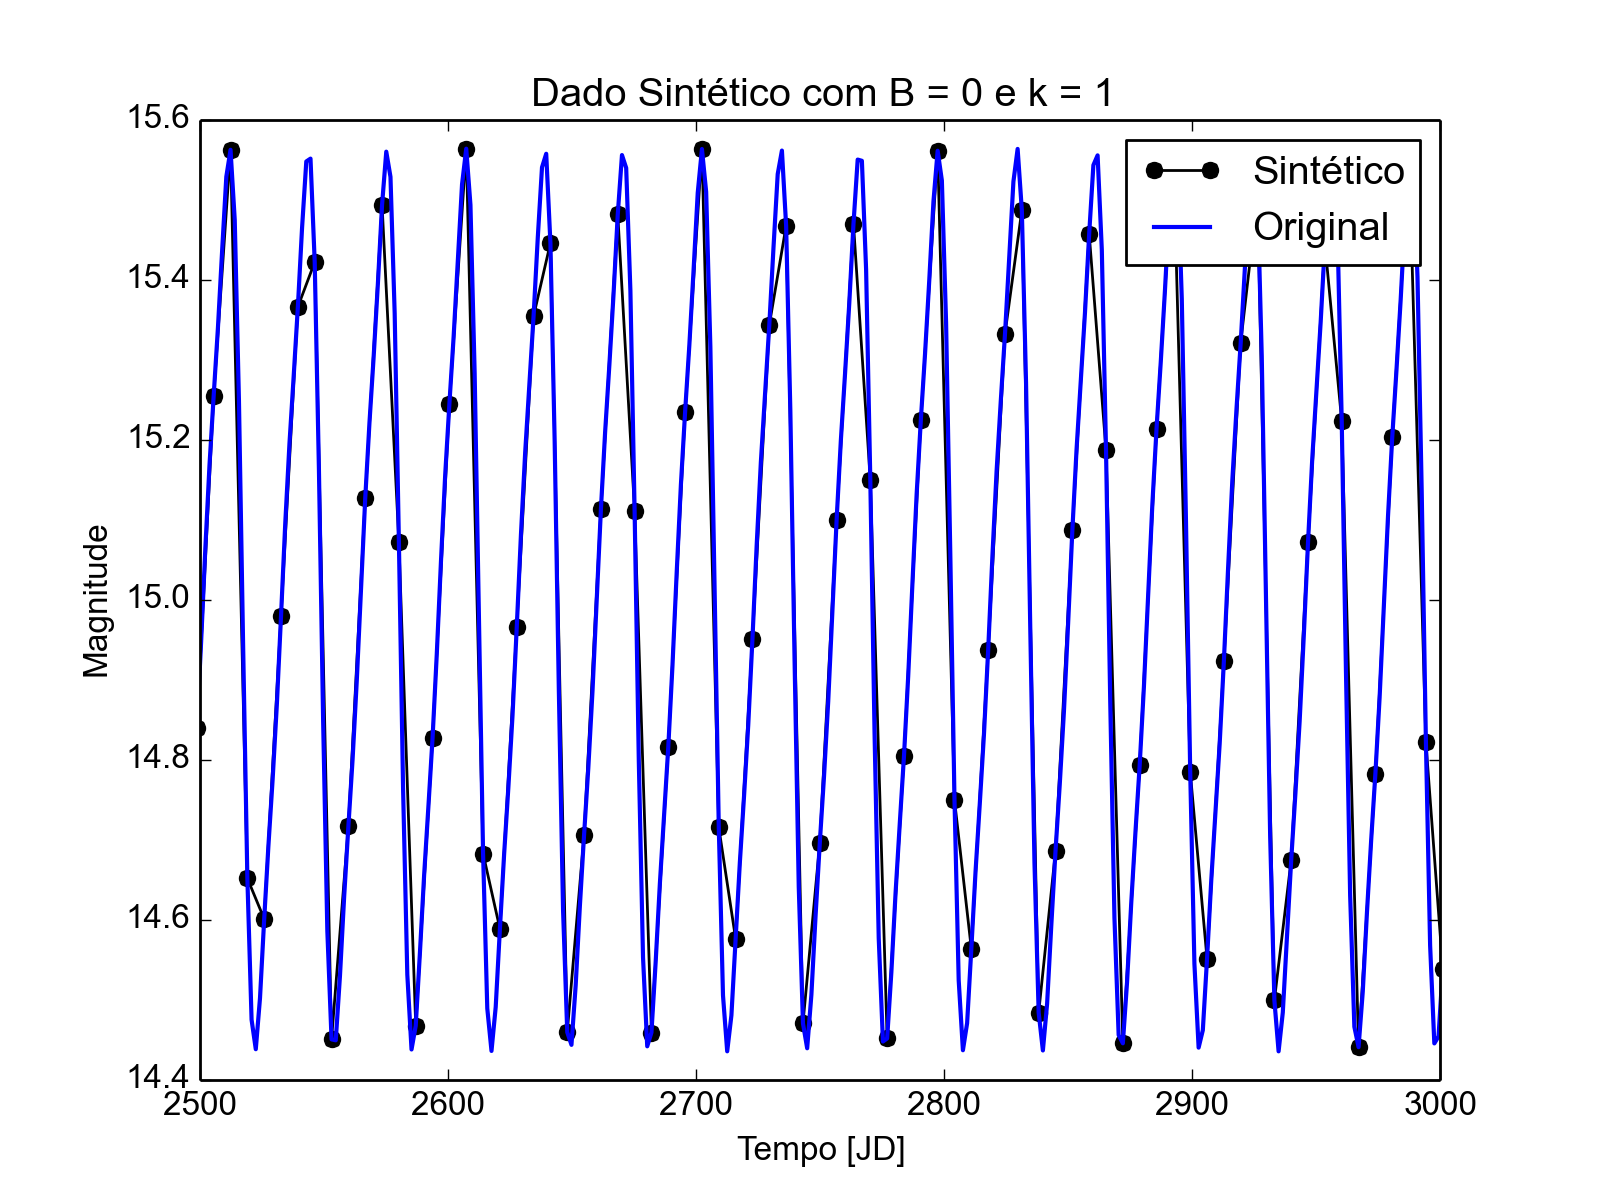
\includegraphics[scale=0.33]{dado_sintetico_0_ruido_1_amos.png}
%   \caption{amostragem padrão}
%   \label{fig:1amos}
% \end{subfigure}%
% \begin{subfigure}{.5\textwidth}
%   \centering
%   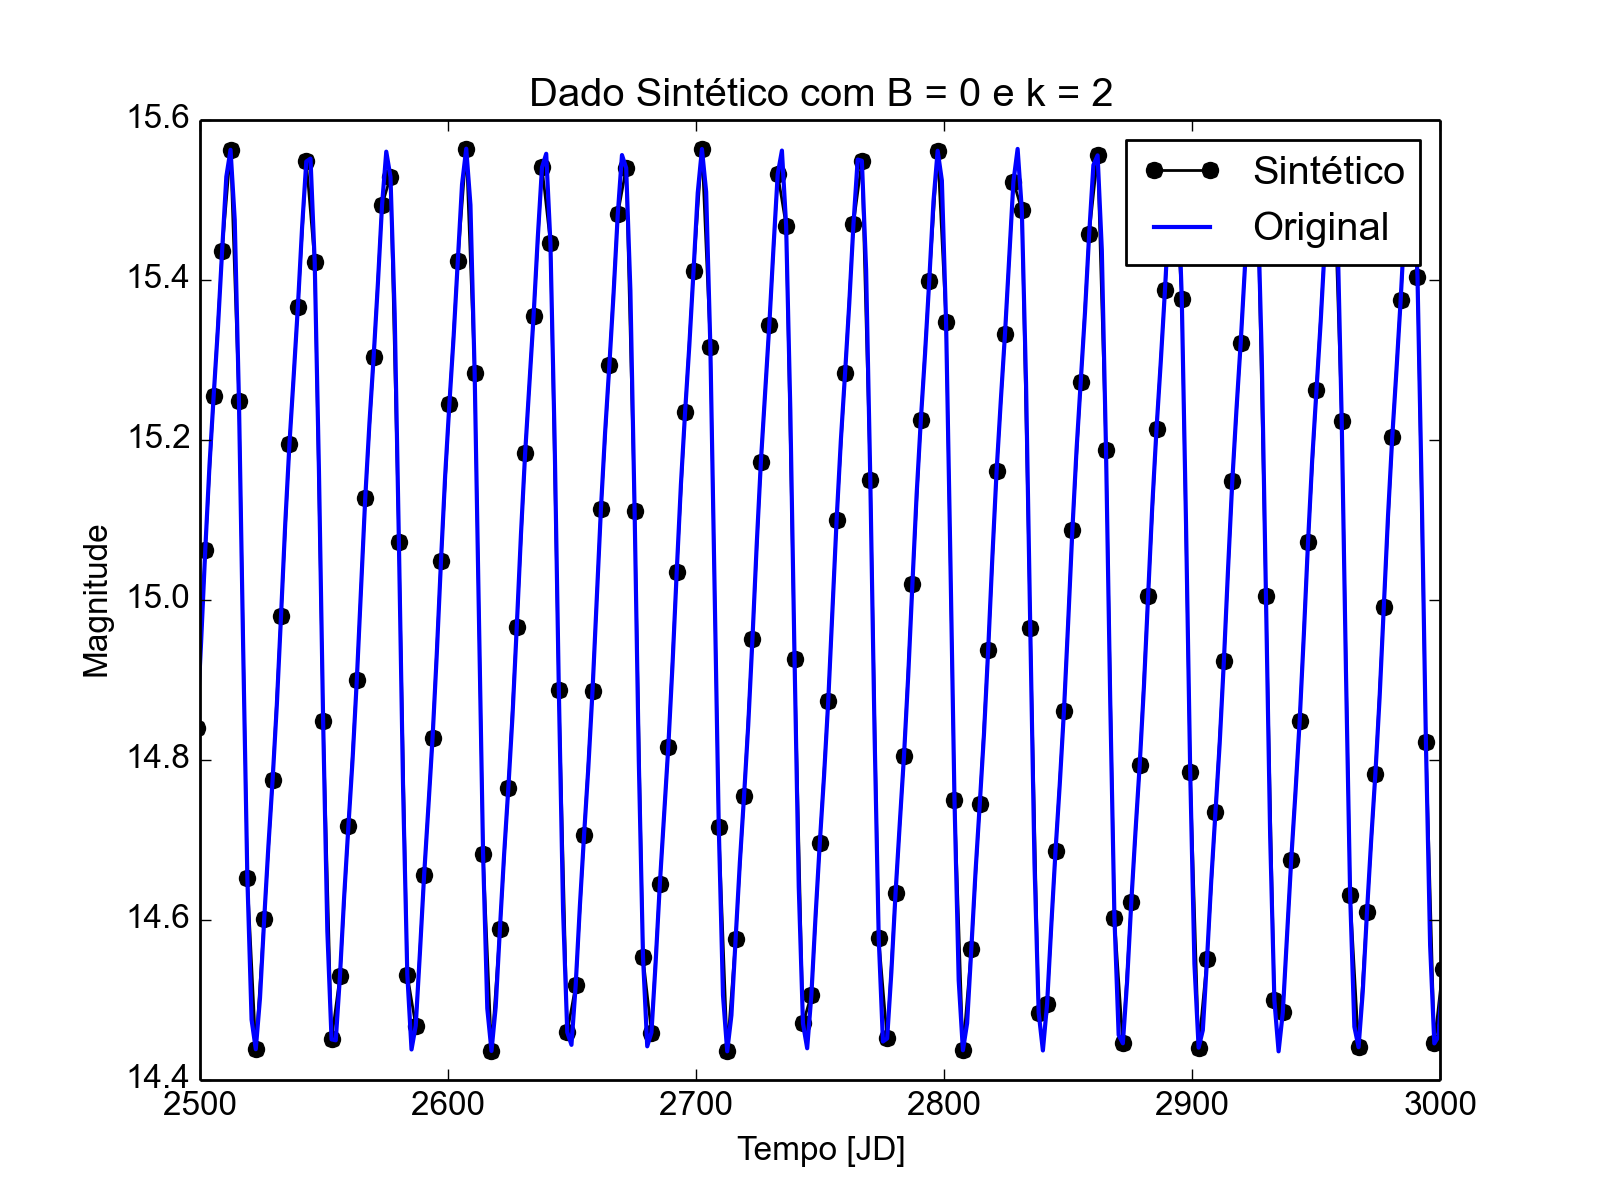
\includegraphics[scale=0.33]{dado_sintetico_0_ruido_2_amos.png}
%   \caption{$n=2$}
%   \label{fig:2amos}
%   \end{subfigure}
% \caption{Exemplos curva de luz sintética}
% \end{figure}
% \end{frame}

% \begin{frame}{Exemplos de Dados Sintéticos}
% \begin{figure}
% \begin{subfigure}{.5\textwidth}
%   \centering
%   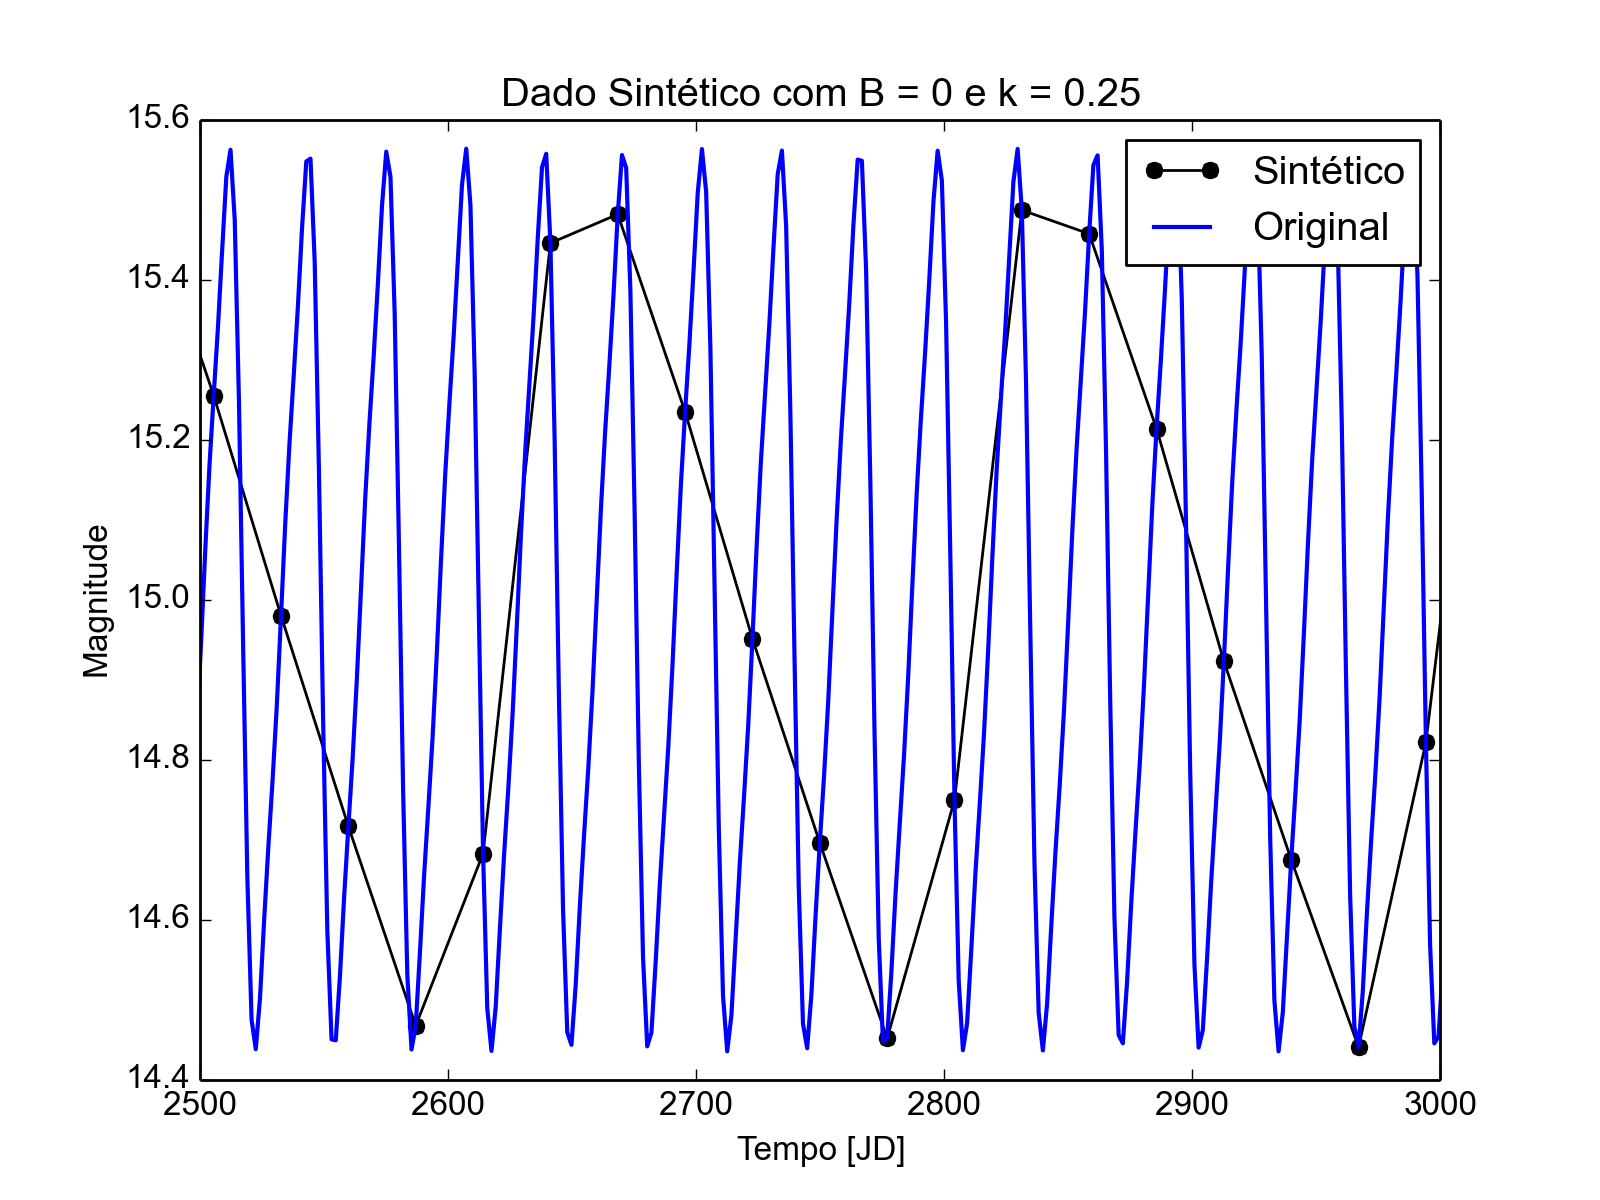
\includegraphics[scale=0.33]{dado_sintetico_0_ruido_0_25_amos.png}
%   \caption{$n=1/4$}
%   \label{fig:025amos}
% \end{subfigure}%
% \begin{subfigure}{.5\textwidth}
%   \centering
%   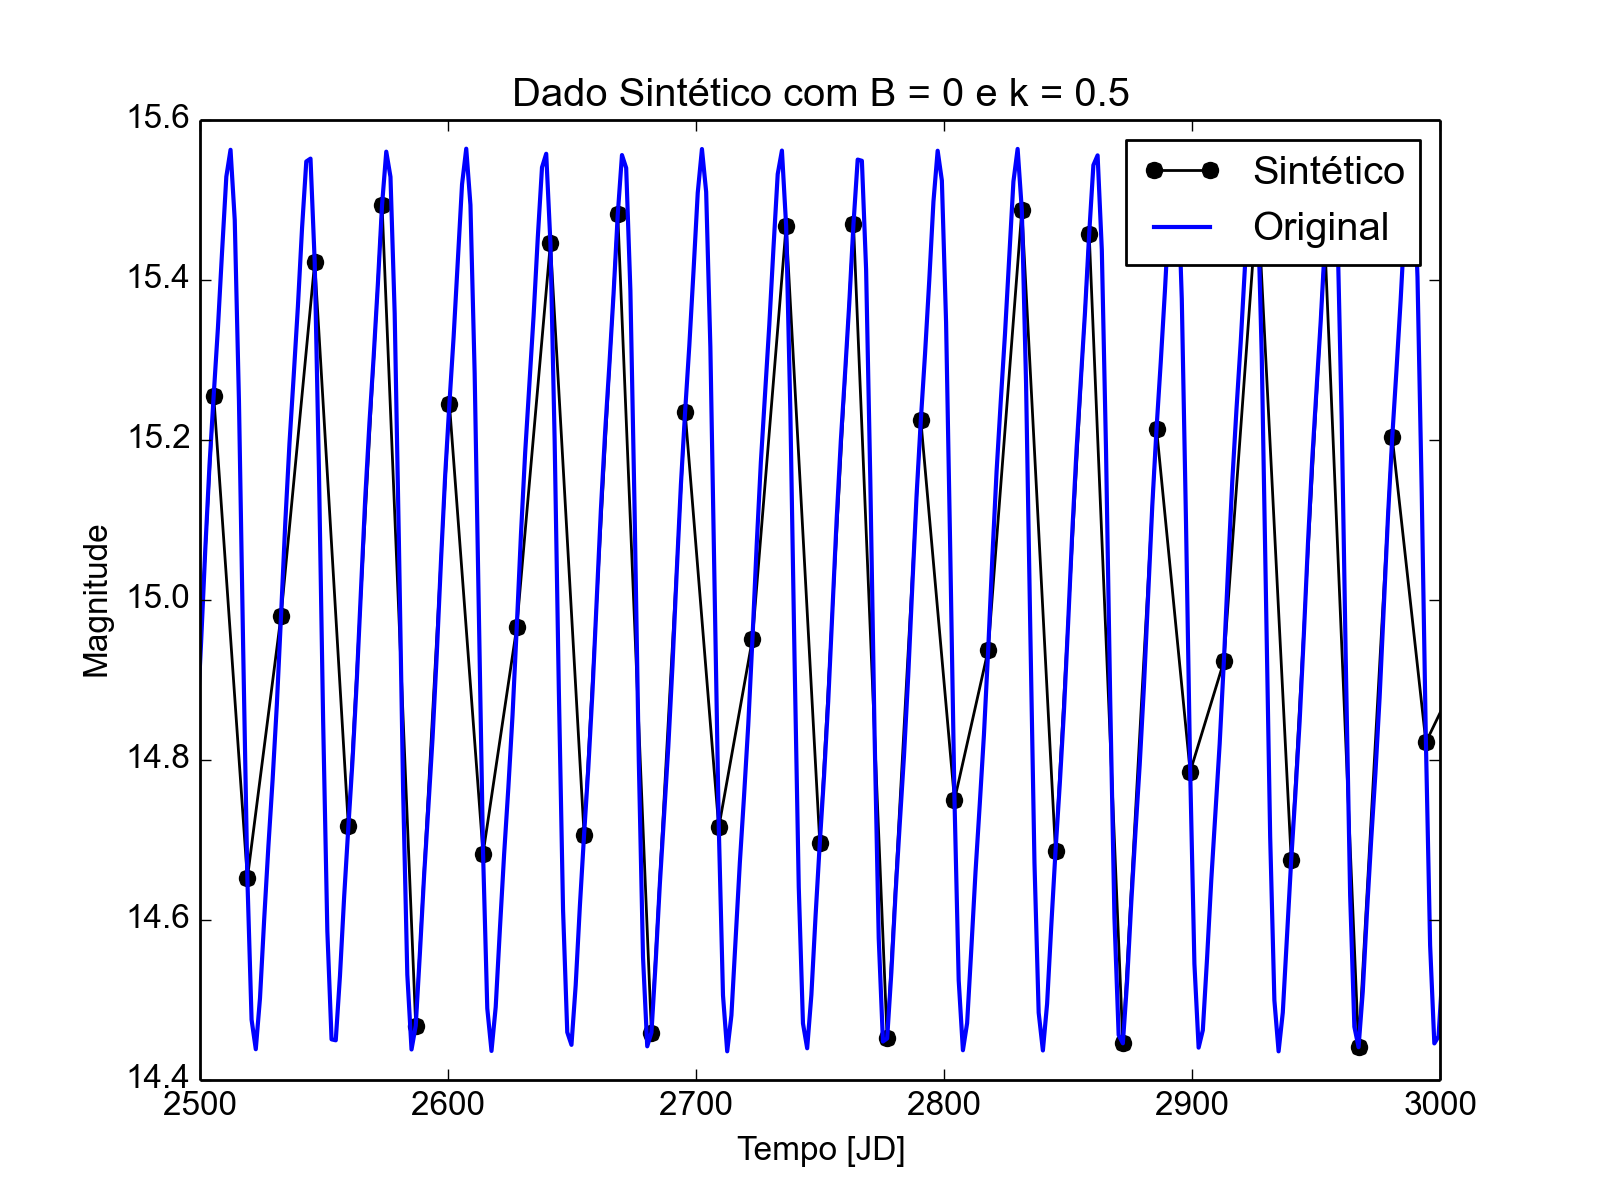
\includegraphics[scale=0.33]{dado_sintetico_0_ruido_0_5_amos.png}
%   \caption{$n=1/2$}
%   \label{fig:05amos}
%   \end{subfigure}
% \caption{Exemplos curva de luz sintética}
% %\label{fig:exemplo_curva_luz}
% \end{figure}

% \end{frame}



\end{document}
